\documentclass[10pt]{article}

\usepackage{times}
\usepackage{natbib}
\usepackage{alltt}
\usepackage[usenames,dvipsnames]{color}
\definecolor{orange}{rgb}{1,0.5,0}

% page setup.
\topmargin -0.7cm
\oddsidemargin 0.2cm
\textwidth 16cm 
\textheight 21cm
\footskip 1.0cm

\usepackage{fancyhdr}

% sets up an environment for the abstract to your paper.
\newenvironment{sciabstract}{\begin{quote} \bf}{\end{quote}}

\if x\pdfoutput\undefined   
\usepackage[dvips]{graphicx}   
\else   
\usepackage[pdftex]{graphicx}
\pdfcompresslevel=9   
\fi   
\usepackage{epstopdf}
%\usepackage{lineno}\linenumbers*[1]
%\usepackage{epsfig}
\usepackage{subfigure,amsmath,amsfonts}
\graphicspath{{./graphics/}}

%\renewcommand\refname{References}

\newcounter{lastnote}
\newenvironment{scilastnote}{%
\setcounter{lastnote}{\value{enumiv}}%
\addtocounter{lastnote}{+1}%
\begin{list}{\arabic{lastnote}.}{\setlength{\leftmargin}{.22in}}{\setlength{\labelsep}{.5em}}}{\end{list}}


\title{\bf Relax: Nonlinear Postseismic Relaxation\\in the Fourier Domain}

\author
{User's Manual\\
\\
\normalsize{Sylvain Barbot (sbarbot@ntu.edu.sg)}\\
\normalsize{Earth Observatory of Singapore, Nanyang Technological University}\\
}

\date{Oct. 11th, 2011, last revision April. 17th, 2014}

\begin{document} 


\thispagestyle{empty}
\begin{figure}[!h]
\centering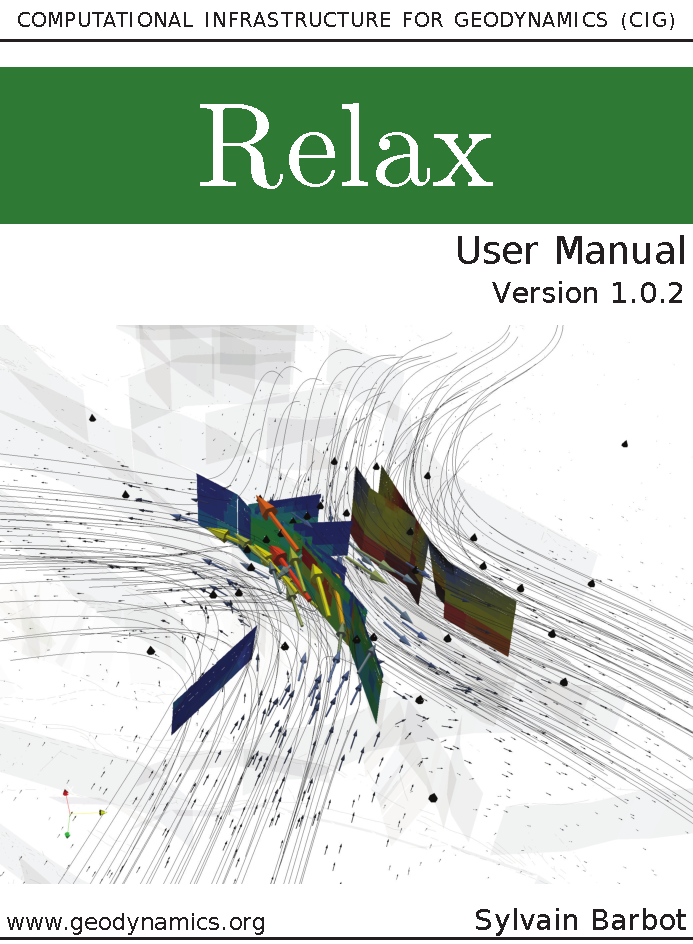
\includegraphics[width=15.092cm]{cover.pdf}
\end{figure}
\pagebreak

\maketitle 


\vspace{1cm}


\pagestyle{fancy}
\cfoot{\thepage}

\section{Introduction}

The open-source program Relax evaluates the displacement and stress in a half space with gravity due to dislocations~\citep[e.g.,][]{okada92}, Mogi sources~\citep{mogi58}, and surface tractions; and the nonlinear time-dependent deformation that follows due to power-law rheology materials in the bulk and/or rate-strengthening friction faults. The numerical method is based on a Fourier-domain elastic Green's function~\citep{barbot+09b,barbot&fialko10a} and an equivalent body-force representation of co-seismic and post-seismic deformation processes~\citep{barbot+09a,barbot&fialko10b}. Application of the method for the 2004 Mw\,6 Parkfield earthquake can be found in the work of~\cite{barbot+09a} and \cite{bruhat+11}. A coupled model of afterslip and laterally-heterogeneous viscoelastic flow following the 1999 Mw\,7.6 Chi-Chi earthquake using Relax is described by~\cite{rousset+12}.

The possible applications for the earthquake-cycle modeling include i) co-seismic displacement and Coulomb stress calculation, ii) quasi-static stress transfer between earthquakes due to a postseismic transient, iii) modeling of postseismic transients including nonlinear rheologies and multiple mechanisms, iv) cycle of multiple earthquakes and spin-up models, v) loading cycle of lakes or the monsoon, vi) generation of viscoelastic Green's functions for kinematic inversions of geodetic time series.

\section{Acknowledgments}
We are greatly thankful for the help of Yuri Fialko and Walter Landry, who contributed to the coming about of the software. We appreciate the efforts of Lucile Bruhat, Yaru Hsu, Mikhail Kogan, Zhen Liu and Baptiste Rousset for testing an earlier version of the code. The support of CIG is greatly appreciated.


\vspace{2.5cm}
%\footnote{sdfl}
\let\thefootnote\relax\footnotetext{The cover image is a Paraview visualization of the displacement field produced by the 1992 Mw 7.3 Landers earthquake from the coseismic slip model of~\cite{fi04c}. The coseismic shear stress on the Hector Mine faults is shown on the far right. The streamlines and the vectors indicate the direction of motion. The shadowed neighboring faults are from UCERF 2 and the prisms indicate continuous GPS stations. The model and the visualization can be reproduced using the material provided in the examples.}


\pagebreak

\tableofcontents

\pagebreak

\section{Theoretical background}

\subsection{Green's function}
The approach used in Relax to evaluate the three-dimensional displacement in a half space is to solve for the displacement field, for static deformation, or the velocity field, for quasi-static problems, using the elastic Green's function. Static deformation caused by earthquakes and time-dependent processes such as viscoelastic flow, poroelastic rebound and fault afterslip can be represented by equivalent body forces and surface tractions so the methods consists, without loss of generality, in finding the displacement and stress caused by an arbitrary distribution of body forces $f_i$ and surface tractions subjected to a mixed boundary condition with buoyancy. Consider the inhomogeneous Navier's equation
%
\begin{equation}\label{eqn:inhomogeneous_navier_equation}
\mu\left(\frac{\alpha}{1-\alpha}u_{j,ij}+u_{i,jj}\right)+f_i=0
\end{equation}
%
where $\mu$ is the shear modulus, $\alpha$ is a dimensionless parameter that can be expressed in terms of the Lam\'{e}'s parameters or the Poisson's ratio
\begin{equation}
\alpha=\frac{\lambda+\mu}{\lambda+2\mu}=\frac{1}{2(1-\nu)}~,
\end{equation}
$u_i$ is the displacement (or velocity) and $f_i$, the internal body force (or force per unit time), subjected to the surface boundary condition
%
\begin{equation}\label{eqn:surface_boundary_condition}
q_i+\sigma_{ij}n_j+\Delta\rho\,g\,u_3 n_i=0,\qquad x_3=0
\end{equation}
%
with $\sigma_{ij}$ the Cauchy stress tensor, $n_i=(0,0,-1)$ the surface normal vector and $q_i(x_1,x_2)$, the prescribed surface traction. The solution displacement that satisfies eq.~(\ref{eqn:inhomogeneous_navier_equation}) and (\ref{eqn:surface_boundary_condition}) can be decomposed into a homogeneous and a particular contribution
\begin{equation}\label{eqn:decomposition_particular_general}
u_i=u_i^h+u_i^p
\end{equation}
where the displacement field $u_i^h$ is a solution of the homogeneous Navier's equation
%
\begin{equation}\label{eqn:homogeneous_navier}
\alpha\,u^h_{j,ij}+(1-\alpha)\,u^h_{i,jj}=0
\end{equation}
with inhomogeneous surface boundary conditions and the particular solution $u^p$ satisfies eq.~(\ref{eqn:inhomogeneous_navier_equation}) regardless of the surface boundary condition. 
%
The particular solution can be obtained in the Fourier domain
%
\begin{equation}\label{eqn:full_space_fourier_solution}
\hat{u}^p_i(k_1,k_2,k_3)=\left\{
\begin{aligned}
&0~,  & &k_1=k_2=k_3=0\\
&\frac{1}{\mu}\frac{(1-\alpha)\,k_lk_l\,\delta_{ij}-\alpha\,k_ik_j}{4\pi^2(k_lk_l)^2}\,\hat{f}_j~, & &\text{otherwise}\\
\end{aligned}
\right.
\end{equation}
where the $k_i$ are the wavenumbers and the hats correspond to the Fourier transform of the corresponding variables. The zero wavenumber component of the Fourier solution corresponds to a rigid-body displacement and does not correspond to an elastic deformation. The temporary solution requires the following correction to satisfy the traction boundary condition. 
\begin{equation}\label{eqn:fourier_domain_solution}
\begin{aligned}
\hat{u}_1^h(k_1,k_2,x_3)&=\big[-2B_1\beta^2+\alpha\,\omega_1\,(B_1\omega_1+B_2\,\omega_2)(1+\beta\,x_3)\\
&\qquad\qquad\qquad+~\alpha\,i\omega_1\beta\,B_3(1-\alpha^{-1}+\beta x_3)\big]\,e^{-\beta\,x_3}\\
\hat{u}_2^h(k_1,k_2,x_3)&=\big[-2B_2\beta^2+\alpha\,\omega_2\,(B_1\,\omega_1+B_2\omega_2)(1+\beta\,x_3)\\
&\qquad\qquad\qquad+~\alpha\,i\omega_2\beta\,B_3(1-\alpha^{-1}+\beta x_3)\big]\,e^{-\beta\,x_3}\\
\hat{u}_3^h(k_1,k_2,x_3)&=\alpha\,\beta^2\big[\,i\left(\omega_1B_1+\omega_2B_2\right)x_3\\
&\qquad\qquad\qquad-~B_3\left(\alpha^{-1}+\beta\,x_3\right)\big]\,e^{-\beta\,x_3}\\
\end{aligned}
\end{equation}
where we have used $\beta=2\pi\left(k_1^2+k_2^2\right)^{1/2}$. The values of the $B_i$ are chosen to satisfy the inhomogeneous boundary condition
\begin{equation}
\begin{aligned}
B_1(k_1,k_2)&=\frac{\hat{p}_1(k_1,k_2)}{2\mu\,\beta^3}\\
B_2(k_1,k_2)&=\frac{\hat{p}_2(k_1,k_2)}{2\mu\,\beta^3}\\
B_3(k_1,k_2)&=\frac{\beta\,\hat{p}_3(k_1,k_2)-i(1-\alpha)[\omega_1\hat{p}_1(k_1,k_2)+\omega_2\hat{p}_2(k_1,k_2)]}{2\mu\,\alpha\,\beta^3(\beta+\gamma)}
\end{aligned}
\end{equation}
where the effective traction $\hat{p}_i$ incorporates external traction and buoyancy
\begin{equation}\label{eqn:last_degree_freedom}
\hat{p}_i(k_1,k_2,x_3=0)=\hat{t}^p_i+\Delta\rho\,g\,\hat{u}^p_3\,n_i+\hat{q}_i
\end{equation}
%
with
%
\begin{equation}\label{eqn:integral1}
\hat{u}_3^p(k_1,k_2,x_3=0)=\int_{-\infty}^\infty\hat{u}^p_3(k_1,k_2,k_3)\,dk_3
\end{equation}
and
\begin{equation}\label{eqn:integral2}
\hat{t}^p_i(k_1,k_2)=\mu\int_{-\infty}^\infty\left(k_j\hat{u}^p_i+k_i\hat{u}^p_j-\frac{1-2\alpha}{1-\alpha}\,k_l\hat{u}^p_l\delta_{ij}\right)\,n_j\,dk_3
\end{equation}


The formulation (\ref{eqn:fourier_domain_solution}-\ref{eqn:integral2}) is a solution for the elastic deformation in a homogeneous half space with mixed boundary condition. The solution is evaluated analytically in the Fourier domain and a space-domain solution is obtained with a fast Fourier transform. The advantage is that the performance of the computation scales as $N\,\log\,N$, where $N$ is the number of samples in the grid, independently of the number of dislocation. The discrete Fourier transform also introduces periodicity in the solution. In many cases, this is not a desired feature, so the boundaries of the computational domain should be as far as possible from the domain of interest.

\subsection{Time integration}

The time stepping in Relax is done by linearizing the time advance using the Runge-Kutta numerical integration scheme with an adaptive time steps.
For viscoelastic flow and afterslip, the instantaneous strain rate is a function of stress only so that one can write
\begin{equation}
\dot{\epsilon} = f(t,\epsilon)
\end{equation}
The second-order Runge-Kutta numerical integration to integrate the $y'=f(t,y)$ can be summarized as follows:
\begin{equation}
\begin{aligned}
y_{n+1} &= y_n + k_2\\
k_1 &= h * f(t_n, y_n)\\
k_2 &= h * f(t_n + h, y_n + k_1)
\end{aligned}
\end{equation}
The scheme is second-order accurate, so reducing the time steps help avoiding numerical instabilities.

\subsection{Equivalent body-force representation of dislocation}

The slip on a finite fault can be represented by a linear combination of force moments and surface tractions~\citep{aki&richards80a}. The method is quite popular in seismology to represent an earthquake as a double-couple point source, but the same representation holds for finite sources.
%
\begin{figure*}[h]
\centering
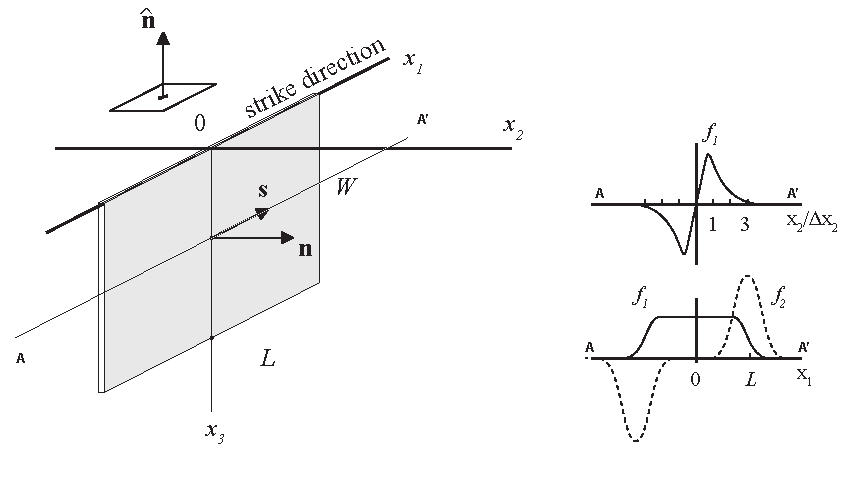
\includegraphics[width=0.6\textwidth]{geometry_finite_fault}
\caption{\small Equivalent body force for a vertical strike-slip fault of length $L$ and width $W$. The fault slip is tapered with the $\Omega$ function of Eq.~(\ref{eqn:omega}).}
\label{fig:geometry_finite_fault}
\end{figure*}
%
It is possible to express analytically the spatial distribution of body forces and surface traction for a patch of rectangular fault slip. For a vertical rectangular strike-slip fault of length $L$ and width $W$ (Figure~\ref{fig:geometry_finite_fault}), the body force representation is
\begin{equation}\label{eqn:body-force}
\begin{aligned}
f_1(x_1,x_2,x_3)&=-G~ \Omega_\beta\!\left(\frac{x_1}{L}\right)\frac{\partial}{\partial x_2}\delta_T\!\left(x_2\right)\Omega_\beta\!\left(\frac{x_3}{W}\right)\\
f_2(x_1,x_2,x_3)&=-G~ \frac{\partial}{\partial x_1}\Omega_\beta\!\left(\frac{x_1}{L}\right)\delta_T\!\left(x_2\right)\Omega_\beta\!\left(\frac{x_3}{W}\right)\\
f_3(x_1,x_2,x_3)&=0
\end{aligned}
\end{equation}
where the function $\Omega_\beta(x)$ is the tapered boxcar parameterized with roll-off parameter $\beta$
\begin{equation}\label{eqn:omega}
\begin{aligned}
\Omega_{\beta}(x)&=%
\left\{\begin{aligned}%
&1\text{,}\quad|x|<\frac{1-2\beta}{2(1-\beta)}\\
&\cos\left(\pi\frac{(1-\beta)|x|-\frac{1}{2}+\beta}{2\beta}\right)^2
\text{,}\\
& \qquad\qquad\qquad\frac{1-2\beta}{2(1-\beta)}<|x|<\frac{1}{2(1-\beta)}& &\\
&0\text{,}\quad\text{ otherwise}%
\end{aligned}\right.
\end{aligned}
\end{equation}
and the function $\delta$ is the numerical equivalent to the Dirac's delta function, for example
\begin{equation}
\delta_T(x)=\frac{1}{T\sqrt{2\pi}}\exp\!\left(-\frac{x^2}{2T^2}\right)
\end{equation}
In Relax, the fault thickness is chosen to be the sampling size $T=\Delta x$. A similar relation can be found for faults of arbitrary orientation. The generalization simply involves rotations and translations. 

\pagebreak
\section{Setting up the program}

\subsection{Introduction}
The Relax code is written in Fortran90 with a few I/O functions written in C. The performance of the code depends greatly on the efficiency of the discrete Fourier transform being used. The program can work with the Cooley-Tukey FFT algorithm, for which the source code is provided. For better performance, it is recommended to use the FFT native to the computer environment. The program can readily use the SGI, the FFTW and the Intel MKL FFTs. While we have found that the Intel MKL FFT provides the most efficient calculation, the package provided by the CIG web site implements FFTW.

Both the post-processing and the storage of the simulation are greatly facilitated by writing output files in the cross-platform NetCDF binary format used by the Generic Mapping Tools (GMT). GMT is convenient to rapidly display the simulation results as it is computed, transform the output into other formats or projections (for example, to project the displacement into the Radar line of sight of a satellite to compare with synthetic aperture radar data), make animations and communicate results. Although Relax can output in ASCII format, it is recommended to link the code to the GMT 4.5 libraries. A suite of GMT-based post-processing scripts are available in the \verb`util` directory and require the GMT binaries to be installed in your system.

The output of the simulation can be projected on the fly to geographic coordinates, which is convenient to communicate results to others in a global coordinate system. In Relax, this is performed with the Proj4 library (Proj4.7.1 or higher). It is recommended to install these libraries on your system to facilitate post processing.

Examples input files can be found in the \verb'examples' directory for many earthquakes with published slip distribution models. The directory \verb'examples/tutorials' includes simple directions to evaluate models and carry out post processing and mapping. The man page (type \verb'man relax' in a terminal) provides a thorough description of every input item, and provides additional examples.

\subsection{Running}


The binary packages provided on the CIG website contain everything needed to run simulations.  After unpacking the packages, open a terminal (or, in Windows, a Command Prompt) and run the setup script
\begin{alltt}
{\color{orange}source setup.sh}  # for Linux and Mac on bash
{\color{orange}source setup.csh} # for Linux and Mac on csh
{\color{orange}setup.bat}        # for Windows
\end{alltt}
You should get the response
\begin{alltt}
{\color{NavyBlue}Ready to run Relax.}
\end{alltt}
On Linux and Mac, you can check which shell is running (\verb`bash` or \verb`csh`) by typing the command \verb`ps -p $$` in a terminal.

On shared memory machines, such as most modern laptops and desktops, it is possible to run the code in parallel using \verb'openmp'. The number of CPU's used is the maximum number of threads allowed by the machine, or the number found in the environment variable \verb'OMP_NUM_THREADS'. To change the value, type
\begin{alltt}
{\color{orange}export OMP_NUM_THREADS=4} # for Linux and Mac
{\color{orange}set OMP_NUM_THREADS=4}    # for Windows
\end{alltt}
on the command line. This command affects all other programs running
in this session. On Linux or Mac machines, to set the number for a
specific run, prepend the variable definition to your command
\begin{alltt}
{\color{orange}OMP_NUM_THREADS=4 relax --option}
\end{alltt}

Some examples of simple calculations are provided in the \verb'examples/tutorials' directory. For instance, to run the first example, change into the \verb'examples/tutorials' directory and run
\begin{alltt}
{\color{orange}./run1.sh}  # for Linux and Mac
{\color{orange}./run1.bat} # for Windows
\end{alltt}
Alternately, on Windows, you can double-click on \verb'run1.bat' from the file browser.

\section{Modeling a deformation scenario}

The computation is performed in a uniform Cartesian grid (see Figure~\ref{fig:computation_grid}). The grid is defined by the number of nodes in the three directions (\verb'SX1', \verb'SX2', \verb'SX3'). The code is designed to deal with dimensions that are powers of two only: 128, 256 or 512, for example. The spatial extent of the computational domain depends on the sampling intervals, (\verb'DX1', \verb'DX2', \verb'DX3'). The horizontal extent of the computational grid is \verb'SX1*DX1' and \verb'SX2*DX2' , in the $x_1$ and $x_2$ directions, respectively. In the depth direction, the computational domain extends from \verb'0' to \verb'SX3*DX3/2'. The coordinate system is right handed, with $x_1$ pointing north, $x_2$ pointing east, and $x_3$ pointing down. 

All the parameters that control the simulation in the input file are assumed to be in S.I. units. That is, lengths are in meters (m), slip is in meters (m), time is in seconds (m), the elastic moduli are in Pascals (Pa). The user is responsible for making the choice of parameters self consistent. For earthquake cycle simulations, it is common to use km, MPa and year for distance, stress, and time units, respectively.

To ensure accurate models, the rule of thumb is to have the domain at least ten times the characteristic dimension of the source, or to have any edge of the computational grid about five fault lengths away from a fault tip. Another constraint that ensures good sampling, is to allow for at least five samples per fault. These two constraints can be satisfied simultaneously by maximizing the number of nodes, at the expense of computer memory.
%
\begin{figure*}[h]
\centering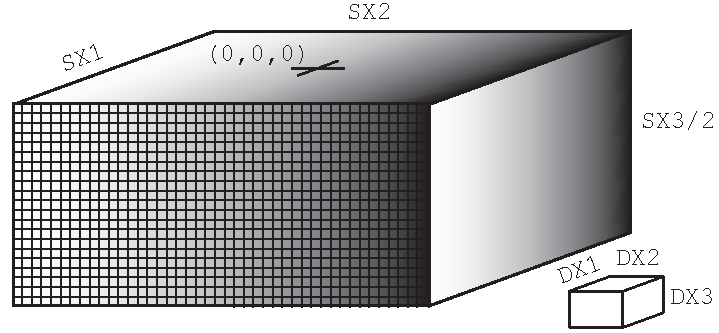
\includegraphics[width=0.6\textwidth]{computational_grid.pdf}
\caption{The discretized half space. The origin of the reference system is at the center of the surface. The modeled half space dimension is $-\Delta x_1\times\text{sx}_1/2$ to $\Delta x_1\times(\text{sx}_1-1)/2$ in the $x_1$ direction, $-\Delta x_2\times\text{sx}_2/2$ to $\Delta x_2\times(\text{sx}_3-1)/2$ in the $x_2$ direction and $0$ to $\Delta x_3\times(\text{sx}_3-1)/2$ in the $x_3$ (depth) direction.}
\label{fig:computation_grid}
\end{figure*}
%

\subsection{Fault geometry}
Many simulations imply the relaxation of the stress perturbation from a coseismic rupture. A rupture model consists in a collection of slip patches that discretize the fault geometry and the slip distribution.
%
\begin{figure*}[h]
\centering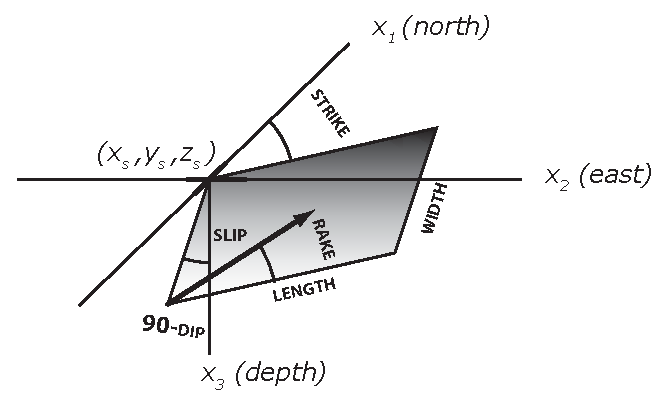
\includegraphics[width=0.6\textwidth]{geologic_fault.pdf}
\caption{Geologic model of slip on a fault. The fault is described by the position of its top tip, its length in the along-strike direction, width in the down-dip direction, its strike angle and its dip angle. The rake indicates the orientation of slip.}
\label{fig:geologic_fault}
\end{figure*}
%
Every slip patch is described by a geologic representation, as shown in Figure~\ref{fig:geologic_fault}. A fault segment is modeled by its length in the along-strike direction, its width in the down-dip direction, the position of the top tip ($x_s, y_s$, and $z_s$) and its strike and dip angles. By convention, an observer located at the top fault tip and oriented in the strike direction would face the fault trace and would have the fault dipping to his right for a dip angle between $0^\circ$ and $90^\circ$. This is the same convention used by \cite{okada92}, \cite{wang+03a} and \cite{wang+06a}. In Relax, to avoid high frequency oscillations near a stress concentration (the so-called Gibbs phenomenon), the slip distribution is smoothed near the fault tip. The amplitude of smoothing is controlled by a roll-off parameter going from $\beta=0$ for no smoothing to $\beta=0.5$ for strong smoothing. A value of $\beta=0.2$ ensures stability of the computation. The seismic moment is conserved for all smoothing values. There is a default value of the smoothing parameter defined at the beginning of the input file
\begin{alltt}
# dx1,dx2,dx3,beta (0-0.5),nq
0.5 0.5 0.5 {\color{orange}0.2} 2
\end{alltt}
but it can be amended for each fault patch. In the following excerpt from an input file, all the fault patches use the smoothing parameter $\beta=0.2$:
\begin{alltt}
# no slip   xs     ys   zs length width strike dip   rake
   1 1.34 14.2 -45.43 10.0    5.6  4.94  132.7  91 -114.7
   2 1.89 10.4 -41.31 10.0    5.6  4.94  132.7  91 -151.8
   3 0.46 14.2 -45.41  6.5   3.74  3.53  132.7  91 -150.6
\end{alltt}
but some patches (here, only the second) can be forced to use another value (here, $\beta=0.5$) as follows:
\begin{alltt}
# no slip   xs     ys   zs length width strike dip   rake beta
   1 1.34 14.2 -45.43 10.0    5.6  4.94  132.7  91 -114.7
   2 1.89 10.4 -41.31 10.0    5.6  4.94  132.7  91 -151.8  {\color{orange}0.5}
   3 0.46 14.2 -45.41  6.5   3.74  3.53  132.7  91 -150.6
\end{alltt}

\subsection{Depth-dependent constitutive parameters}

The Fourier method used by Relax to solve the displacement field and the quasi-static velocity field implies homogeneous elastic moduli in the half space. However, all other inelastic or physical parameters, such as viscosity, friction properties and stress, can vary arbitrarily in the domain. Relax assumes a background depth dependence for these variables. These properties can be modified locally to simulate slabs, ductile zone, or reproduce the gross features of a geological structure. 

Let's look at how to define a viscosity profile for a creme br\^{u}l\'{e}e model, with an elastic plate over a viscoelastic half space. First, note that the Relax input file requires the reference strain rate $\dot{\gamma}_0=\mu/\eta$, instead of the viscosity $\eta$. This is convenient because first, for a purely elastic material, $\dot{\gamma}_0=0$, and second, $\dot{\gamma}_0$ is just the reciprocal of the Maxwell relaxation time $t_m=1/\dot{\gamma}_0$, so one can easily think in terms of time scales of relaxation, instead of viscosities. The default model is elastic, so it is only necessary to indicate where the lithosphere changes from elastic to viscoelastic
\begin{alltt}
# number of linear viscous interfaces (where viscosity changes)
{\color{orange}1}
# no depth gammadot0 cohesion
{\color{orange}   1  30.0       0.1      0.0}
\end{alltt}
Here, we have defined a viscoelastic substrate that extents from 30\,km depth down to the bottom of the computational domain. Assuming that the time units are in year, we have define a uniform viscosity giving rise to a Maxwell time $t_m=1/0.1=10\,$yr.

Let's look at how to define a viscosity profile for a jelly sandwich model, with a viscoelastic lower crust, a competent, elastic upper mantle, and a viscoelastic asthenosphere. The description of the depth variations of the model is written in a similar way to the PREM model in seismology.
\begin{alltt}
# number of linear viscous interfaces for a jelly sandwich strength model
{\color{orange}5}
# no depth gammadot0 cohesion
{\color{orange}   1  15.0       0.1      0.0}
{\color{orange}   2  30.0       0.1      0.0}
{\color{orange}   3  30.0       0.0      0.0}
{\color{orange}   4  70.0       0.0      0.0}
{\color{orange}   5  70.0       0.2      0.0}
\end{alltt}
Here, the lower crust relaxes with a Maxwell time of $t_m=10\,$yr, and the asthenosphere with a Maxwell time of $t_m=5\,$yr. There is no need to specify the viscosity in the upper 15\,km, which is assumed infinite.




\subsection{Lateral variations of viscosity}
Subducting slabs and shear zones below a transform boundary are examples of major structural elements that introduce lateral variations in viscosity in the lithosphere. Including these elements in the Earth structure is done using ductile zones, which are rectangular regions where the viscosity is modified from the background, depth-dependent, value. The volume where the viscosity changes is defined similarly to a fault (using start position, length, width, strike and dip), but a additional thickness parameter indicates how the volume is extruded from the central plane (Fig.~\ref{fig:geologic_zone}).

%
\begin{figure*}[h]
\centering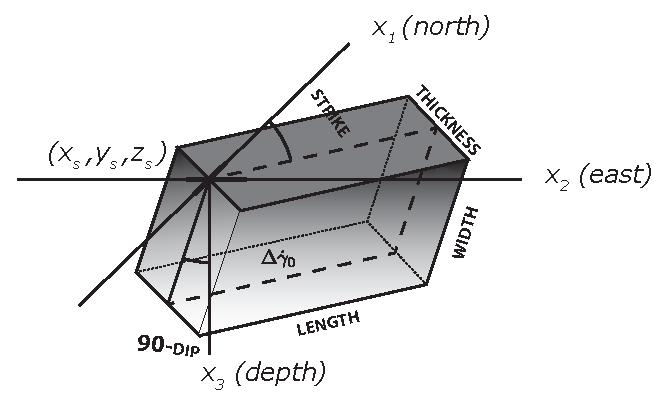
\includegraphics[width=0.6\textwidth]{geologic_zone.pdf}
\caption{Geometry of a ductile zone anomaly. The ductile zone is described by the position of the tip of the central plane (length in the strike direction, width in the dip direction, strike and dip angles). The thickness parameter indicates how the rectangular volume is extruded from its center plane. The $\Delta\dot{\gamma}_0$ parameter adds to the background value of the fluidity.}
\label{fig:geologic_zone}
\end{figure*}
%


Let's look at how to define a viscosity profile where the depth of the brittle-ductile transition changes across a geological boundary. We start with an elastic plate overriding a viscoelastic half space with a uniform brittle-ductile transition depth of 15\,km with a Maxwell time of $t_m=1\,$yr.
\begin{alltt}
...
# number of linear viscous interfaces
{\color{orange}1}
# no depth gammadot0 cohesion
{\color{orange}   1  15.0         1      0.0}
# number of linear ductile shear zones
{\color{orange}1}
# no dgammadot0 x1  x2 x3 length width thickness strike dip
{\color{orange}   1         -1  0   0 10    200     5       200     90  90}
...
\end{alltt}
We then add a large volume abutting the center of the computational volume, where we modify the fluidity from $\dot{\gamma}_0=1\,$yr$^{-1}$ to $\dot{\gamma}_0=0$, using $\Delta\dot{\gamma}_0=-1\,$yr$^{-1}$. As a null fluidity corresponds to elastic behavior, the brittle-ductile transition occurs 5\,km deeper going west to east across the $x_1$ (north-south) axis. The geometry of a slab can be obtained by modifying the strike and dip angles. Changing the strike of the ductile zone from 90 to 0$^\circ$ would make the transition occur from south to north. If the background and anomalous fluidities add to a negative, unphysical, value, the sum is corrected to null, and the result is an effective elastic property. 

Realistic structures can be accounted for from structural data using a large quantity of ductile anomalies tuned to observations. Consider the case of the Sunda subduction slab where the top of the elastic slab is described by a series of fault segments:
\begin{alltt}
# no         x1         x2        x3 length     width   strike    dip   rake
001 -1008.18345 976.507098  8.540000 50.000 50.094787 -53.2903 3.5252 76.733
002 -969.881237 944.367717  8.922983 50.000 50.089914 -51.1015 3.4335 78.917
003 -931.579015 912.228337  9.414930 50.000 50.131393 -50.4005 4.1491 79.626
004 -893.276793 880.088956 10.365896 50.000 50.219974 -48.2526 5.3646 81.783
005 -854.974571 847.949576 11.813879 50.000 50.404913 -46.9655 7.2673 83.089
006 -816.672349 815.810195 11.651879 50.000 50.416558 -46.1198 7.3703 83.930
007 -778.370126 783.670815 11.301228 50.000 50.406643 -44.0841 7.2827 85.948
008 -740.067904 751.531434 11.463158 50.000 50.410988 -41.9865 7.3212 88.029
009 -701.765682 719.392054 11.242973 50.000 50.406957 -40.3630 7.2855 89.639
010 -663.463460 687.252674 10.615908 50.000 50.373596 -40.3511 6.9824 89.651
011 -625.161238 655.113293 10.455476 50.000 50.350356 -40.8200 6.7630 89.185
...
\end{alltt}
which is saved in the file \verb'sunda.flt'. A three-dimensional model of the elastic slab can be constructed by extending the fault segments into volumes. Lets consider a 80\,km thick slab. We start with a depth-dependent model with visco-elastic relaxation below 80\,km:
\begin{alltt}
# number of linear viscous interfaces for elastic plate
{\color{orange}1}
# no depth gammadot0 cohesion
{\color{orange}   1  80.0       1.0      0.0}
# number of linear ductile zone
{\color{orange}0}
\end{alltt}
and let's add the down-going slab:
\begin{alltt}
# number of linear viscous interfaces for elastic plate
{\color{orange}1}
# no depth gammadot0 cohesion
{\color{orange}   1  80.0       1.0      0.0}
# number of linear ductile zone
{\color{orange}`grep -v "#" sunda.flt | wc`}
# nb dgammadot0   x1   x2   x3   length   width   thickness   strike   dip
{\color{orange}`grep -v "#" sunda.flt | awk '{print NR,-10,$2,$3,$4,$5,80,$6,$7,$8+90}'`}
...
\end{alltt}
The last line creates a list of blocks extending the slab interface down and reducing the fluidity by a large number ($-10\,$yr$^{-1}$) to set the fluidity to 0 and the viscosity to infinity. The slab geometry is shown in Fig.~\ref{fig:sunda}.

%
\begin{figure*}[h]
\centering
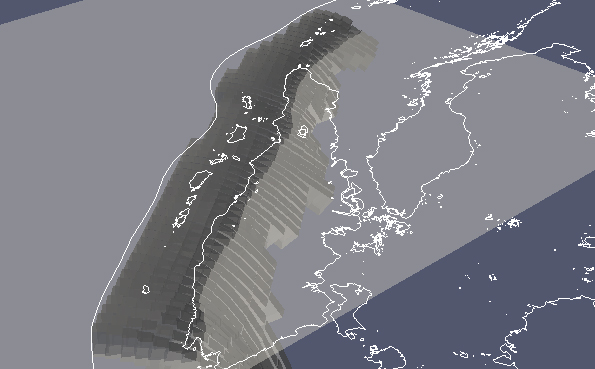
\includegraphics[width=\textwidth]{sunda.jpg}
\caption{\small Three-dimensional viscoelastic structure for the Sunda down-going slab. The opaque interface represent an elastic lithosphere extended at depth by the cubic boxes (ductile zones). The mantle wedge is below Sumatra.}
\label{fig:sunda}
\end{figure*}
%



\pagebreak
\section{Examples}

\subsection{Simple coseismic model}

Let's consider first the simplest input model to compute the static deformation due to a left-lateral strike-slip fault. Figure \ref{input:simple_coseismic} shows the entire input file required to describe the simulation. Note how the code is called, with the command \verb'relax --no-proj-output <<EOF'. In unix, it means that all the text that appears after this line, until the three characters \verb'EOF' are found, is considered as input for the program. In this case, the program is called with the option \verb'--no-proj-output' to indicate that the output does not have to be projected in lat/lon coordinates. It can be useful to call the program with the \verb'--dry-run' option, i.e.,
\begin{alltt}
relax --no-proj-output {\color{orange}--dry-run} <<EOF
# SX1,SX2,SX3 (grid size)
256 256 256
# dx1,dx2,dx3 (km),beta (0-0.5),nq (2)
0.5 0.5 0.5 0.2 2
...
\end{alltt}
to check the geometry of the model. In this case, all the fault patches, the slip distribution and the spatial extent of the grid are exported in the \verb'.vtp' format, which is a standard 3-D geometry format that can be read with such visualization tools as Paraview (\verb'http://www.paraview.org').

Unless the \verb'--no-vtk-output' option is used, the program exports the displacement field of the entire computational domain in the VTK Legacy binary format for 3-D visualization. For long time-dependent simulation, this output can consume large amount of disk space and it can be useful to discard it with the \verb'--no-vtk-output' option. The stress field is also exported in this format by default. This is cancelled with \verb'--no-stress-output', but that option cancels out any stress output in GMT format as well.

\begin{figure}
\begin{alltt}
relax --no-proj-output <<EOF
# SX1,SX2,SX3 (grid size)
{\color{orange}256 256 256}
# dx1,dx2,dx3 (km),beta (0-0.5),nq (2)
{\color{orange}0.5 0.5 0.5 0.2} 2
# origin position & rotation
0 0 0
# observation depths for displacement and for stress
{\color{NavyBlue}0 5}
# output directory (all output written here)
output_directory
# lambda (MPa), mu (MPa), gamma (1/km)
{\color{orange}3e4 3e4 8.33e-4}
# integration time, time step and scaling
{\color{orange}0 -1 1}
# number of viscous observation slice
0
# number of observation points
0
# number of Coulomb patches
0
# number of prestress interfaces
0
# number of linear viscous interfaces
0
# number of power-law viscous interfaces
0
# number of friction faults
0
# number of interseismic loading strike-slip and opening
0
0
# number of coseismic events (when slip distribution is prescribed)
1
# number of shear dislocations (strike-slip and dip-slip faults)
1
# no slip  xs ys zs length width strike dip rake
{\color{orange}   1    1 -10  0  0     10    10      0  90    0}
# number of tensile cracks
0
# number of dilatation sources
0
# number of surface traction
0
EOF
\end{alltt}
\caption{Input parameters to compute the coseismic deformation due to a left-lateral strike-slip fault with $L=W=10\,$km. The gravity wavelength is defined as $\gamma=(1-\nu) \rho g/\mu$ where $\nu$ is Poisson's ratio, $\rho$ is the density of the crust and $g$ is the acceleration of gravity. The program provides the displacement field and the stress field in multiple formats.}\label{input:simple_coseismic}
\end{figure}

The standard output of the program is shown in Figure~\ref{input:out_coseismic}. It repeats the details of the input file and adds information such as the recommended maximum sampling size. After the computation, it also outputs one line corresponding to the first time step. It can be useful to save the standard output of the calculation to document what was computed. To do so, one can use the following unix pipeline
\begin{alltt}
{\color{orange}ODIR=output_directory}

relax <<EOF --no-proj-output --no-stress-output{\color{orange} | tee $ODIR/in.param}
# SX1,SX2,SX3 (grid size)
256 256 256
# dx1,dx2,dx3 (km),beta (0-0.5),nq (2)
0.5 0.5 0.5 0.2 2
# origin position & rotation
0 0 0
# observation depths for displacement and for stress
{\color{NavyBlue}0 5}
# output directory
{\color{orange}$ODIR}
# lambda (MPa), mu (MPa), gamma (1/km)
...
\end{alltt}
\begin{figure}
\begin{alltt}
# ----------------------------------------------------------------------------
#      nonlinear postseismic relaxation with Fourier-domain Green function
#      * Intel MKL implementation of the FFT
#      * parallel OpenMP implementation with 016/016 threads
#      * export to GRD format
#      * export to VTK format
#      {\color{NavyBlue}* export to longitude/latitude text format cancelled (--no-proj-output)}
# ----------------------------------------------------------------------------
# grid dimension (sx1,sx2,sx3)
  256  256  256
# sampling (dx1,dx2,dx3), smoothing (beta, nyquist)
  5.00E-1  5.00E-1  5.00E-1  2.00E-1  2.00E+0
# origin position (x0,y0) and rotation
  0.00E+0  0.00E+0  0.00E+0
# observation depth (displacement and stress)
  0.00E+0  5.00E+0
# output directory
 output_directory (time report: output_directory/time.txt)
# lambda, mu, gamma (gamma = (1 - nu) rho g / mu)
  3.00E+04  3.00E+04  8.33E-04
# time interval, (positive time step) or (negative skip, scaling)
  0.00E+0 (output every 001 steps, dt scaled by 1.00E+0)
# number of observation planes
    0
...
# number of events
    1
# number of coseismic strike-slip segments
    1
# ----------------------------------------------------------------------------
# no.     slip       xs       ys       zs  length   width strike   dip   rake
# ----------------------------------------------------------------------------
001  1.00E+0 -1.00E+1  0.00E+0  0.00E+0 1.00E+1 1.00E+1    0.0  90.0    0.0
# ----------------------------------------------------------------------------
# number of coseismic tensile segments
    0
# number of coseismic dilatation point sources
    0
# number of surface loads
    0
# {\color{NavyBlue}max sampling size (hor.,vert.): 4.00E+0 4.00E+0}
# ----------------------------------------------------------------------------
coseismic event 001
 I  |   Dt   | tm(ve) | tm(pl) | tm(as) |     t/tmax     | power  |  C:E^i |
{\color{NavyBlue}000* 0.00E+00 0.00E+00 0.00E+00 0.00E+00 0.00E+00/0.00E+0 0.00E+00 3.08E+06}
\end{alltt}
\caption{Output of the Relax program for the input parameters shown in Figure \ref{input:simple_coseismic}. The Relax output can also serve as an input so it can be useful to save it for documentation purposes and to help reproduce past results.}
\label{input:out_coseismic}
\end{figure}

To visualize the coseismic displacement at the surface, it is convenient to use the script \verb'grdmap.sh'. The plotting routine \verb'grdmap.sh' provided with the code and numerous other post-processing scripts can be used to analyze the modeled scenario. The unix script \verb'grdmap.sh', a wrapper around GMT programs, produces map views of any grid but is optimized to work with the three-dimensional output of Relax.
\begin{alltt}
{\color{NavyBlue}grdmap.sh -b -30/30/-30/30 -p -0.05/0.05/0.001 -v 0.5 \textbackslash
       -u "m" -e erpatch.sh output_directory/000}
\end{alltt}
where the \verb'-b' option defines the boundary of the map in the GMT format W/E/S/N, the \verb'-p' option defines the range of the color scale for the vertical displacements, the \verb'-v' option defines the length of the vectors for the horizontal displacement, the "-u" option defines the unit of the color scale, and the "-e" option call the additional script \verb'erpatch.sh' to plot the spatial extent of the fault on the map. The last argument \verb'output_directory/000' refers to the prefix of all GMT binary files associated with the index \verb'000'. Any file prefix followed by \verb'-north.grd', \verb'-east.grd' and \verb'-up.grd' can be used in this manner. To look at an individual file, for example the stress component $\sigma_{12}$ at 5\,km depth, simply use
\begin{alltt}

{\color{NavyBlue}grdmap.sh -b -30/30/-30/30 -p -500/500/1 \textbackslash
       -u "kPa" -e erpatch.sh output_directory/000-s12.grd}
\end{alltt}
For this command to work, it is assumed that \verb'grdmap.sh' and \verb'erpatch.sh' are both located in a directory listed in the \verb'$PATH' environment variable, such as \verb'/usr/local/bin'.

The coseismic slip distribution of a real earthquake can be a long and detailed description of the source coming from an inversion of geophysical data. To include these models and conform them to the format required by the Relax program, it is convenient to use other unix tricks, such as \verb'awk', \verb'wc' and the use of variables, for instance, if the source is described in the file \verb'src.dat', but the file missing a line counter and the units in meters, one can alter it as follows
\begin{alltt}
...
# number of coseismic events
1
# number of shear dislocations
{\color{orange}`wc src.dat`}
# no slip  xs ys zs length width strike dip rake
{\color{orange}`awk '{\textbraceleft}BEGIN{\textbraceleft}s=1e3{\textbraceright}{\textbraceleft}print NR,$1/s,$2/s,$3/s,$4/s,$5/s,$6/s,$7,$8,$9{\textbraceright}' src.dat`}
# number of tensile cracks
0
# number of dilatation sources
0
# number of surface traction
0
EOF
\end{alltt}
The inclusion of unix commands in the input file allows more complex operations, such as filtering out data, shift, rotation and scaling of models, and others. An example complex coseismic slip distribution for the 1992 Mw 7.3 Landers earthquake can be found in the \verb'examples/mojave' directory.

\subsection{Simple viscoelastic model}

Let's extend our simple coseismic model to include a viscoelastic relaxation in a substrate below 30\,km. To do so, we need to specify a rheology at depth and indicate how long to simulate the relaxation. Relax allows two simultaneous viscoelastic relaxation mechanisms, one from a linear rheology
\begin{equation}\label{eqn:viscoelastic}
\dot{\gamma}^{\text{linear}}=\dot{\gamma}_0\frac{\tau}{\mu}
\end{equation}
where $\dot{\gamma}^{\text{linear}}$ is the amplitude of the linear viscoelastic strain and $\dot{\gamma}_0$ is a reference strain rate; and another from a power-law rheology
\begin{equation}
\dot{\gamma}^{\text{power-law}}=\dot{\gamma}_0\left(\frac{\tau}{\mu}\right)^{n}
\end{equation}
where $n$ is the power exponent (usually in the range $n=2-5$). In this example, we only use the linear rheology. Choosing a viscosity with a Maxwell time of $t_m=1/\dot{\gamma}_0=1$\,yr, we want to compute 20 relaxation times with a time step of $\Delta t=0.1\,$yr. This scenario is specified with the following input lines

\begin{alltt}
...
# elastic moduli and gravity parameter
3e4 3e4 8.33e-4
# integration time, time step
{\color{orange}20 0.1}
# number of observation planes
0
# number of observation points
0
# number of Coulomb patches
0
# number of prestress interfaces
0
# number of linear viscous interfaces
{\color{orange}1}
# no depth gammadot0 cohesion
{\color{orange}   1  30.0       1.0      0.0}
# number of linear ductile zones
{\color{orange}0}
# number of powerlaw viscous interfaces
0
...
\end{alltt}
Note that the time step asked by the program is only the output time step, that is, at what time to output the result. Internally, an optimal time step is always evaluated and the real time step used for the calculation is the smallest of either the internally evaluated value or the time step required to produce an output every multiple of the required time step. The internally evaluated value is always $\Delta t^{\text{internal}}=t_m/10$. Prescribing the output time step can only reduce the computational time step. Note that is a background viscosity has been established, the program requests so called ``ductile zones", which are finite volumes where the background viscosity is perturbed. These volumes are described similarly to for a fault, but with an extra ``thickness" parameter indicating how the volumes extrudes from the center plane. The standard output of this simulation looks as follows
\begin{alltt}
coseismic event 001
 I  |   Dt   | tm(ve) | tm(pl) | tm(as) |     t/tmax     | power  |  C:E^i |
000* 0.00E+00 0.00E+00 0.00E+00 0.00E+00 0.00E+00/2.00E+1 0.00E+00 3.08E+06
001* {\color{NavyBlue}1.00E-01 1.00E+00} 1.00E+07 1.00E+07 1.00E-01/2.00E+1 {\color{NavyBlue}4.25E+06 3.50E+06}
002* 1.00E-01 1.00E+00 1.00E+07 1.00E+07 2.00E-01/2.00E+1 {\color{NavyBlue}3.92E+06 3.89E+06}
003* 1.00E-01 1.00E+00 1.00E+07 1.00E+07 3.00E-01/2.00E+1 {\color{NavyBlue}3.63E+06 4.26E+06}
004* 1.00E-01 1.00E+00 1.00E+07 1.00E+07 4.00E-01/2.00E+1 {\color{NavyBlue}3.35E+06 4.59E+06}
005* 1.00E-01 1.00E+00 1.00E+07 1.00E+07 5.00E-01/2.00E+1 {\color{NavyBlue}3.10E+06 4.90E+06}
006* 1.00E-01 1.00E+00 1.00E+07 1.00E+07 6.00E-01/2.00E+1 {\color{NavyBlue}2.88E+06 5.19E+06}
007* 1.00E-01 1.00E+00 1.00E+07 1.00E+07 7.00E-01/2.00E+1 {\color{NavyBlue}2.67E+06 5.45E+06}
008* 1.00E-01 1.00E+00 1.00E+07 1.00E+07 8.00E-01/2.00E+1 {\color{NavyBlue}2.48E+06 5.70E+06}
009* 1.00E-01 1.00E+00 1.00E+07 1.00E+07 9.00E-01/2.00E+1 {\color{NavyBlue}2.31E+06 5.93E+06}
010* 1.00E-01 1.00E+00 1.00E+07 1.00E+07 1.00E+00/2.00E+1 {\color{NavyBlue}2.15E+06 6.14E+06}
011* 1.00E-01 1.00E+00 1.00E+07 1.00E+07 1.10E+00/2.00E+1 {\color{NavyBlue}2.00E+06 6.34E+06}
012* 1.00E-01 1.00E+00 1.00E+07 1.00E+07 1.20E+00/2.00E+1 {\color{NavyBlue}1.87E+06 6.53E+06}
013* 1.00E-01 1.00E+00 1.00E+07 1.00E+07 1.30E+00/2.00E+1 {\color{NavyBlue}1.74E+06 6.70E+06}
014* 1.00E-01 1.00E+00 1.00E+07 1.00E+07 1.40E+00/2.00E+1 {\color{NavyBlue}1.63E+06 6.86E+06}
015* 1.00E-01 1.00E+00 1.00E+07 1.00E+07 1.50E+00/2.00E+1 {\color{NavyBlue}1.53E+06 7.01E+06}
016* 1.00E-01 1.00E+00 1.00E+07 1.00E+07 1.60E+00/2.00E+1 {\color{NavyBlue}1.43E+06 7.15E+06}
017* 1.00E-01 1.00E+00 1.00E+07 1.00E+07 1.70E+00/2.00E+1 {\color{NavyBlue}1.34E+06 7.28E+06}
018* 1.00E-01 1.00E+00 1.00E+07 1.00E+07 1.80E+00/2.00E+1 {\color{NavyBlue}1.26E+06 7.40E+06}
019* 1.00E-01 1.00E+00 1.00E+07 1.00E+07 1.90E+00/2.00E+1 {\color{NavyBlue}1.18E+06 7.52E+06}
020* 1.00E-01 1.00E+00 1.00E+07 1.00E+07 2.00E+00/2.00E+1 {\color{NavyBlue}1.11E+06 7.63E+06}
021* 1.00E-01 1.00E+00 1.00E+07 1.00E+07 2.10E+00/2.00E+1 {\color{NavyBlue}1.05E+06 7.73E+06}
022* 1.00E-01 1.00E+00 1.00E+07 1.00E+07 2.20E+00/2.00E+1 {\color{NavyBlue}9.88E+05 7.82E+06}
023* 1.00E-01 1.00E+00 1.00E+07 1.00E+07 2.30E+00/2.00E+1 {\color{NavyBlue}9.32E+05 7.91E+06}
024* 1.00E-01 1.00E+00 1.00E+07 1.00E+07 2.40E+00/2.00E+1 {\color{NavyBlue}8.79E+05 7.99E+06}
025* 1.00E-01 1.00E+00 1.00E+07 1.00E+07 2.50E+00/2.00E+1 {\color{NavyBlue}8.31E+05 8.07E+06}
026* 1.00E-01 1.00E+00 1.00E+07 1.00E+07 2.60E+00/2.00E+1 {\color{NavyBlue}7.85E+05 8.15E+06}
027* 1.00E-01 1.00E+00 1.00E+07 1.00E+07 2.70E+00/2.00E+1 {\color{NavyBlue}7.43E+05 8.22E+06}
028* 1.00E-01 1.00E+00 1.00E+07 1.00E+07 2.80E+00/2.00E+1 {\color{NavyBlue}7.03E+05 8.28E+06}
029* 1.00E-01 1.00E+00 1.00E+07 1.00E+07 2.90E+00/2.00E+1 {\color{NavyBlue}6.66E+05 8.35E+06}
030* 1.00E-01 1.00E+00 1.00E+07 1.00E+07 3.00E+00/2.00E+1 {\color{NavyBlue}6.31E+05 8.40E+06}
031* 1.00E-01 1.00E+00 1.00E+07 1.00E+07 3.10E+00/2.00E+1 {\color{NavyBlue}5.98E+05 8.46E+06}
032* 1.00E-01 1.00E+00 1.00E+07 1.00E+07 3.20E+00/2.00E+1 {\color{NavyBlue}5.67E+05 8.51E+06}
033* 1.00E-01 1.00E+00 1.00E+07 1.00E+07 3.30E+00/2.00E+1 {\color{NavyBlue}5.39E+05 8.56E+06}
034* 1.00E-01 1.00E+00 1.00E+07 1.00E+07 3.40E+00/2.00E+1 {\color{NavyBlue}5.11E+05 8.61E+06}
035* 1.00E-01 1.00E+00 1.00E+07 1.00E+07 3.50E+00/2.00E+1 {\color{NavyBlue}4.86E+05 8.65E+06}
...
\end{alltt}
The standard output indicates the evaluated Maxwell time (if the viscosity is not uniform, the smallest value of the inferred Maxwell time is used) for the viscoelastic rheology, in the \verb'tm(ve)' column. This value should not evolve throughout the calculation. The time step where output is written to disk are shown with an asterisk, such as \verb'014*'. As the output time step corresponds to the computational time step, the value of the displacement, velocity, stress and other variables are output to disk at every time step. The column \verb'power' is important to check the sanity of the calculation. For a relaxation scenario, the power should reduce at each time step. If not the case, it is symptomatic of a numerical integration error. To correct this, decrease the time steps, or the spatial sampling, or both. The last column is the cumulative moment of inelastic deformation and should always increase.

By default, the deformation is written to disk in map view, for mapping with GMT, or in volume, for 3-D rendering with Paraview, at each step. For time dependent problems, it is convenient for certain points in the domain to save the time series of deformation in a single file. To do so, define ``observation points" as follows
\begin{alltt}
...
# number of observation planes
0
# number of observation points
{\color{NavyBlue}3}
# no name       x1       x2       x3
{\color{NavyBlue} 001 GPS1  1.00E+1  0.00E+0  0.00E+0
 002 GPS2  2.00E+1  0.00E+0  0.00E+0
 003 GPS3  3.00E+1  0.00E+0  0.00E+0}
# number of stress observation segments
0
...
\end{alltt}
The observation points are given a four-character name \verb'name' and the time series of displacement and stress is listed in the output file \verb'name.txt'. Using the above example, we obtain
\begin{alltt}
> more output_directory/GPS1.txt
#         t         u1        u2         u3       s11        s12       s13
  0.000E+00 -1.736E-05 1.726E-01 -2.343E-08 1.034E-03 -2.199E+03 4.950E-01
  1.000E-01 -1.738E-05 1.726E-01 -2.356E-08 1.035E-03 -2.198E+03 4.950E-01
  2.000E-01 -1.739E-05 1.727E-01 -2.368E-08 1.036E-03 -2.197E+03 4.951E-01
  3.000E-01 -1.741E-05 1.728E-01 -2.376E-08 1.035E-03 -2.197E+03 4.951E-01
...
\end{alltt}
where we have discarded the last three component of the stress tensor in the interest of space. The observation points list the cumulative displacement and stress, including the initial perturbation from an earthquake and the contribution due to the viscoelastic relaxation.


In many cases, the observation points may be the coordinates of GPS stations in a large network or the ground coordinates of the pixels of a synthetic aperture radar interferogram, or some other image of surface deformation. If the location of the surface points are listed in a file \verb'pos.xy', one can create as many time series with a command such as
\begin{alltt}
...
# number of observation points
{\color{NavyBlue}`wc pos.xy`}
# no name       x1(north)       x2(east)       x3(depth)
{\color{NavyBlue}`awk '{\textbraceleft}printf("\%d G\%03d \%f \%f 0{\textbackslash}n",NR,NR,$2,$1){\textbraceright}' pos.xy`}
# number of stress observation segments
0
...
\end{alltt}
which will create files named \verb'G001.txt', \verb'G002.txt' and so forth, for each point.



\subsection{Simple afterslip model}

Let's use Relax to simulate the deep afterslip that follows a main shock. To do so, we will add a fault below the rupture and assign rate-strengthening properties. We assume that the slip on the fault is governed by a rate-strengthening constitutive law
\begin{equation}
V=2\,\dot{\gamma}_0\,\sinh\frac{\Delta\tau}{(a-b)\sigma}
\end{equation}
where $\Delta\tau$ is the stress perturbation due to the earthquake, which is slowly relaxed, and $(a-b)\sigma$ and $\dot{\gamma}_0$ are constitutive parameters. In general, a good value for $(a-b)\sigma$ is of the order of the stress drop of the earthquake, and perhaps slightly smaller. The dimension-less ratio
\begin{equation}
k=\frac{\Delta\tau}{(a-b)\sigma}~,
\end{equation}
where $\Delta\tau$ is the stress drop, in the range $1\le k\le 7$. Attention, since $\sinh(x)\sim\exp(x)$ for $x\gg1$, too small a value for $(a-b)\sigma$ will make the evaluation of the velocity challenging. In this case the execution will stop with an error message indicating a diagnostic value of $\Delta\tau$ and of $(a-b)\sigma$. The time scale of the afterslip scales with
\begin{equation}
t_m^{\text{afterslip}}\propto\frac{L}{2\,\dot{s}_0}\frac{a\,\sigma}{G}
\end{equation}
where $L$ is the dimension of the creep area. One can use this scaling relationship to choose the parameters and obtain a reasonable time scale. 

An peculiar behavior of this friction law is that the time evolution is non linear, with in some conditions much faster velocities at the early stage of the afterslip transient than at later times. To resolve this numerically, it requires adaptive time steps. To output the simulation at every computational time step, use negative output time steps:
\begin{alltt}
...
# integration time, time step and scaling
{\color{NavyBlue}20 -1 0.5}
...
\end{alltt}
In this case, a third argument is needed to modify the internally-evaluated computational time step (here it will be reduced by a half). For example, to output the solution every 10 computational time steps without altering the internal $\Delta t$ estimate, use
\begin{alltt}
...
# integration time, time step and scaling
{\color{NavyBlue}20 -10 1}
...
\end{alltt}


The definition of an afterslip model includes depth-dependent friction properties and the geometry of a receiver fault. To compute the response of afterslip on a deep extension of the rupture defined in the above examples, use
\begin{alltt}
...
# number of nonlinear viscous interfaces
0
# number of fault creep interfaces
{\color{orange}1}
# no depth   gamma0 (a-b)sig friction cohesion
{\color{orange}   1     0      0.3      1e3      0.6        0}
# number of afterslip planes
{\color{orange}1}
# no  x1 x2 x3 length width strike  dip rake
{\color{orange}   1 -10  0 11     10    10      0   90    0}
# number of inter-seismic strike-slip segments
0
...
\end{alltt}
The standard output reads
\begin{alltt}
coseismic event 001
 I  |   Dt   | tm(ve) | tm(pl) | tm(as) |     t/tmax     | power  |  C:E^i |
000* 0.00E+00 0.00E+00 0.00E+00 0.00E+00 0.00E+00/2.00E+1 0.00E+00 3.08E+06
001* {\color{NavyBlue}1.89E-02} 1.00E+07 1.00E+07 {\color{NavyBlue}3.78E-01} 1.89E-02/2.00E+1 {\color{NavyBlue}1.14E+06 3.10E+06}
002* {\color{NavyBlue}2.76E-02} 1.00E+07 1.00E+07 {\color{NavyBlue}5.53E-01} 4.65E-02/2.00E+1 {\color{NavyBlue}9.47E+05 3.12E+06}
003* {\color{NavyBlue}2.97E-02} 1.00E+07 1.00E+07 {\color{NavyBlue}5.94E-01} 7.62E-02/2.00E+1 {\color{NavyBlue}8.06E+05 3.15E+06}
004* {\color{NavyBlue}2.95E-02} 1.00E+07 1.00E+07 {\color{NavyBlue}5.91E-01} 1.06E-01/2.00E+1 {\color{NavyBlue}7.02E+05 3.17E+06}
005* {\color{NavyBlue}2.94E-02} 1.00E+07 1.00E+07 {\color{NavyBlue}5.88E-01} 1.35E-01/2.00E+1 {\color{NavyBlue}6.22E+05 3.19E+06}
006* {\color{NavyBlue}2.93E-02} 1.00E+07 1.00E+07 {\color{NavyBlue}5.86E-01} 1.64E-01/2.00E+1 {\color{NavyBlue}5.57E+05 3.20E+06}
007* {\color{NavyBlue}2.92E-02} 1.00E+07 1.00E+07 {\color{NavyBlue}5.84E-01} 1.94E-01/2.00E+1 {\color{NavyBlue}5.03E+05 3.22E+06}
008* {\color{NavyBlue}2.91E-02} 1.00E+07 1.00E+07 {\color{NavyBlue}5.82E-01} 2.23E-01/2.00E+1 {\color{NavyBlue}4.57E+05 3.23E+06}
009* {\color{NavyBlue}2.90E-02} 1.00E+07 1.00E+07 {\color{NavyBlue}5.80E-01} 2.52E-01/2.00E+1 {\color{NavyBlue}4.17E+05 3.24E+06}
010* {\color{NavyBlue}2.90E-02} 1.00E+07 1.00E+07 {\color{NavyBlue}5.79E-01} 2.81E-01/2.00E+1 {\color{NavyBlue}3.82E+05 3.25E+06}
011* {\color{NavyBlue}2.89E-02} 1.00E+07 1.00E+07 {\color{NavyBlue}5.78E-01} 3.10E-01/2.00E+1 {\color{NavyBlue}3.52E+05 3.26E+06}
012* {\color{NavyBlue}2.88E-02} 1.00E+07 1.00E+07 {\color{NavyBlue}5.77E-01} 3.38E-01/2.00E+1 {\color{NavyBlue}3.25E+05 3.27E+06}
013* {\color{NavyBlue}2.88E-02} 1.00E+07 1.00E+07 {\color{NavyBlue}5.75E-01} 3.67E-01/2.00E+1 {\color{NavyBlue}3.01E+05 3.28E+06}
...
\end{alltt}
and shows a monotonic decrease of the power and a gradual increase of the time steps.


\subsection{Stress change calculations}
Relax can be used to evaluate the stress change caused by an earthquake or a magmatic intrusion on other faults and structures. There are five ways to look at stress change in Relax: time series at given points, slices, arbitrary cross sections into the domain, three-dimensional visualization in Paraview, and calculation of stress change along an arbitrary number of receiver faults. In addition to providing instantaneous stress change, Relax can provide the time series of stress change due to both the initial source of the deformation and the transient that follows the event. 

By default, Relax exports the displacement and stress as a function of time and space in GMT's .grd format. (Stress export can be cancelled with the \verb'--no-stress-output' command-line option.) In the following example, surface displacements and all stress components at a depth of 5\,km are exported in the .grd format.
%
\begin{alltt}
relax --no-proj-output <<EOF
# SX1,SX2,SX3 (grid size)
256 256 256
# dx1,dx2,dx3 (km),beta (0-0.5),nq (2)
0.5 0.5 0.5 0.2 2
# origin position & rotation
0 0 0
# observation depths for displacement and for stress
{\color{orange}0 5}
...
\end{alltt}
Slices of co-seismic stress change at 5\,km depth are in the files \verb'000-s11.grd', \verb'000-s12.grd', \verb'000-s13.grd', \verb'000-s22.grd', \verb'000-s23.grd' and \verb'000-s33.grd'. These files correspond to the $\sigma_{ij}$ components of the stress tensor. Other components $\sigma_{ji}$ can be obtained taking advantage of the symmetry of the stress tensor ($\sigma_{ij}=\sigma_{ji}$). Following earthquakes, it can be interesting to evaluate the pore pressure change as it drives poro-elastic rebound. The pore pressure change is a function of the change in confining pressure $\sigma_{kk}$, which can be computed as follows using GMT's \verb'grdmath'
\begin{alltt}
{\color{NavyBlue}index=output/000
grdmath $\{index\}-s\{11,22\}.grd ADD $\{index\}-s33.grd ADD = $\{index\}-skk.grd}
\end{alltt}
To better anticipate the extent of the viscoelastic deformation (where will the rocks flow after an earthquake), we can evaluate the norm of the deviatoric stress $\tau$, as it drives viscoelastic flow (eq.~\ref{eqn:viscoelastic}). The deviatoric stress tensor $\sigma'_{ij}$ contains no isotropic component, so we can simply compute its diagonal components as follows
\begin{alltt}
{\color{NavyBlue}grdmath $\{index\}-s11.grd $\{index\}-skk.grd SUB = $\{index\}-s11p.grd
grdmath $\{index\}-s22.grd $\{index\}-skk.grd SUB = $\{index\}-s22p.grd
grdmath $\{index\}-s33.grd $\{index\}-skk.grd SUB = $\{index\}-s33p.grd}
\end{alltt}
The vigor of viscoelastic flow will be controlled by the norm of the deviatoric stress tensor (eq.~\ref{eqn:viscoelastic}) and the direction of the flow will be controlled by how the amplitude of stress projects in different directions. The norm of the deviatoric stress can be evaluated as follows
\begin{alltt}
{\color{NavyBlue}grdmath $\{index\}-s11p.grd 2 POW $\{index\}-s22p.grd 2 POW ADD $\{index\}-s33p.grd \textbackslash 
        2 POW ADD 2 DIV $\{index\}-s12.grd 2 POW ADD $\{index\}-s13.grd 2 POW ADD \textbackslash 
        $\{index\}-s23.grd 2 POW ADD = $\{index\}-tau.grd}
\end{alltt}
For a more subtle look at the dynamics of stress change, we can look at the log of shear stress change (Fig.~\ref{fig:wharton})
\begin{alltt}
{\color{NavyBlue}grdmath $\{index\}-tau.grd LOG10 = $\{index\}-log10-tau.grd}
\end{alltt}
%
\begin{figure*}[p]
\centering
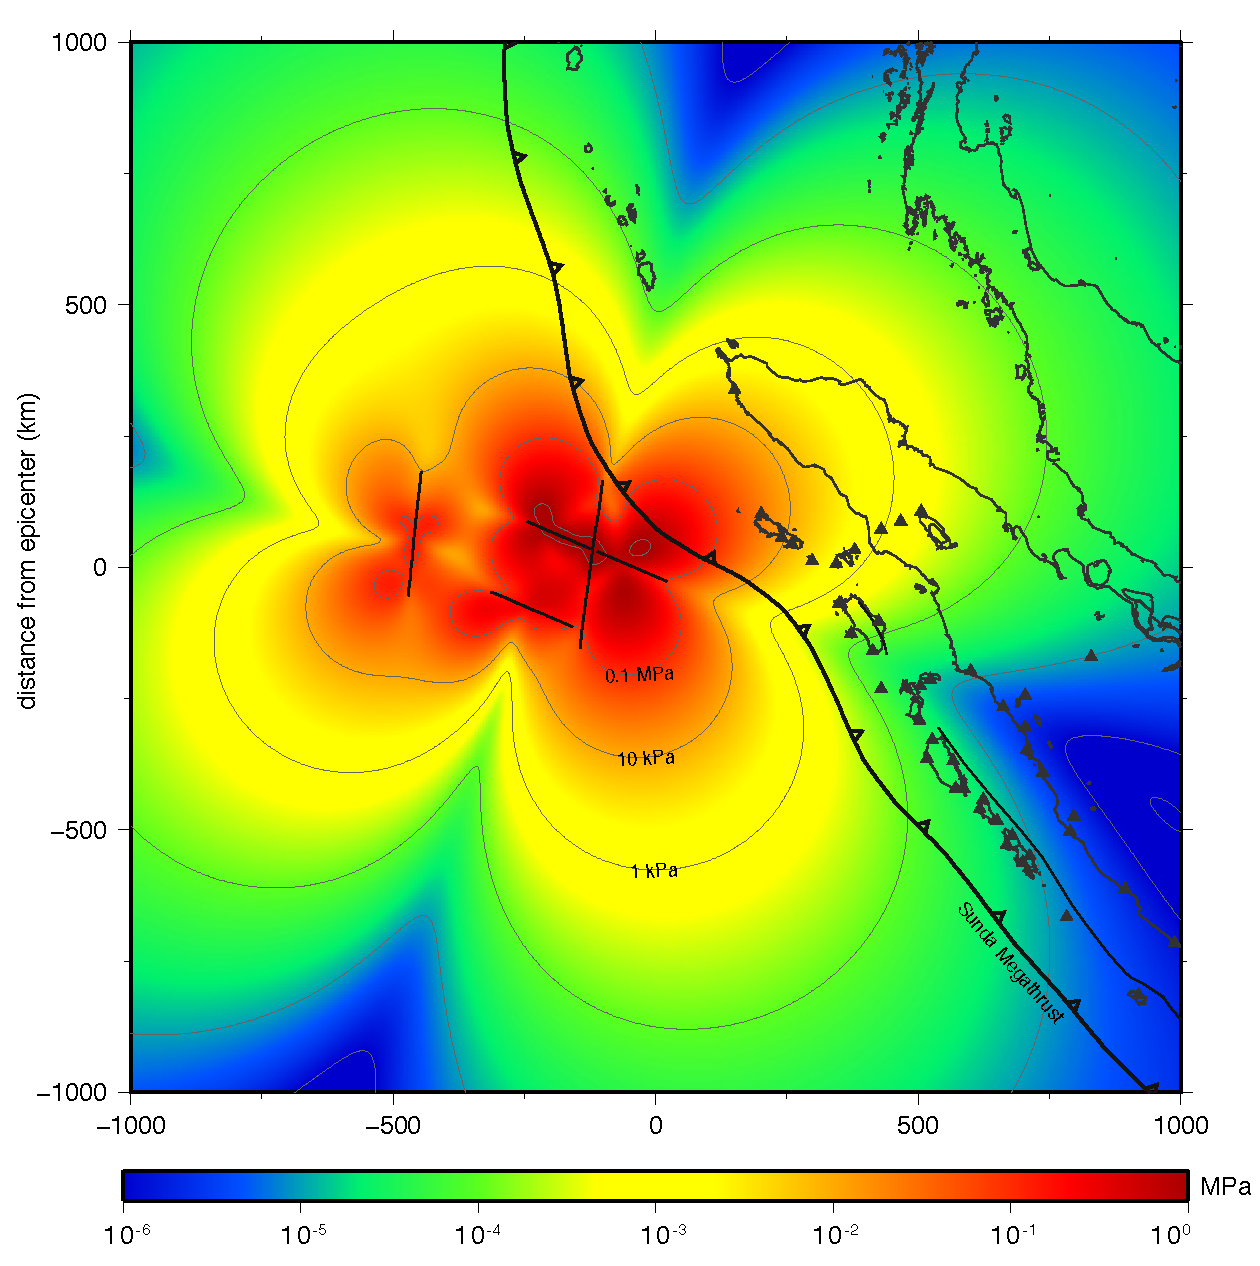
\includegraphics[width=\textwidth]{stress_change_wharton.pdf}
\caption{\small Coseismic stress change at 80\,km depth induced by the 2012 Mw\,8.6 Wharton Basin earthquake from a slip-distribution model by Hill et al. (2014). The map shows the logarithm of the norm of the deviatoric stress change. The Sunda megathrust around Simulue and Banda Aceh, in northern Sumatra, are experiencing significantly more stress change than other regions.}
\label{fig:wharton}
\end{figure*}
%

The files \verb'001-s11.grd', \verb'001-s12.grd', ..., \verb'001-s33.grd' contain the total stress change at time step 1, including both the stress change induced by the original event and the stress change induced by the transient that follows. To look at the stress change due to the relaxation alone, we can isolate it as follows:
\begin{alltt}
{\color{NavyBlue}grdmath 001-s12.grd 000-s12.grd SUB = 001-relax-s12.grd}
\end{alltt}

To look at stress change in three dimensions, we can open \verb'sigma-0000.vtk' in Paraview and look at contours of stress components or compute the deviatoric stress change using the Calculator Filter. Another way is to sample the stress along a cross section using an observation plane:
\begin{alltt}
...
# elastic moduli and gravity parameter
3e4 3e4 8.33e-4
# integration time, time step
20 -1 1
# number of observation planes
{\color{orange}1}
# n     x1     x2 x3 length width  strike dip
{\color{orange}  1  168.5 -438.7  0   1600   160 112.992  90}
...
\end{alltt}
The stress components are then exported in GMT's .grd files \verb'000.op001-s11.grd', \verb'000.op001-s12.grd', ..., \verb'000.op001-s33.grd', where the first index \verb'000' is for the time step and \verb'op001' is for observation plane 1. All the calculations described above are applicable: just define the new index to \verb'index=output/000.op001' before running \verb'grdmath'. An example application of map view and cross sections of stress change calculations can be found in~\cite{rousset+12}.

Cross sections and maps provide a general view of the extent and amplitude of stress change. But it is sometimes useful to look at stress change on receiver faults. This offers the advantage to be able to decompose the stress components in directions relevant to faults: the strike, dip and fault normal directions. Also, receiver faults can have a non planar overall shape, so using receiver faults allows us to follow a complex fault geometry. Receiver faults are defined by their position, dimension, orientation and static coefficient of friction, for example
\begin{alltt}
...
# number of stress observation segments
{\color{orange}1}
# n  x1 x2 x3 length width strike dip friction
{\color{orange}  1 -10  0  0     20    10      0  90      0.6}
...
\end{alltt}
The stress change is calculated at the center of the fault (here that would be 0,0,5). A time series of stress change at the center of the fault can be found in '\verb'cfaults-sigma-0001.txt'. In the case of multiple fault segments, each file will contain all components of the stress tensor, the shear and normal components of the traction vector, the strike- and dip-direction components of the traction vector, the fault-normal component of the traction vector and the Coulomb stress change:
\begin{alltt}
#         t        s11        s12        s13        s22        s23        s33
{\color{NavyBlue}  0.000E+00  2.392E-03  1.583E-03  4.540E-04  4.810E-04  2.366E-04  2.169E-04}
\end{alltt}
and
\begin{alltt}
#       taus       taud        tau       taun    Coulomb
{\color{NavyBlue}-7.224E-04 -7.665E-04  1.053E-03  4.578E-04  4.707E-02}
\end{alltt}
on a single line per time step. The files \verb'rfaults-dsigma-0000.vtp' and \verb'rfaults-dsigma-0000.xy' contain the postseismic stress change on all receiver faults for a given time step for visualization in Paraview and GMT, respectively. The files \verb'rfaults-sigma-0000.vtp' and \verb'rfaults-sigma-0000.xy' contain the cumulative stress change due to both coseismic and postseismic deformation. Together, these files allow us to look at the time series of stress change for a single fault receiver, or look at all the receivers for a given time step. Let's look at an example where we use the same fault as source and receiver:
\begin{alltt}
...
# number of stress observation segments
{\color{orange}`grep -v "#" slip_model.flt | wc`}
# n x1 x2 x3 length width strike dip rake friction
{\color{orange}`grep -v "#" slip_model.flt | awk '\{\$2="";\$9=0.6;print \$0\}'`}
# number of prestress interfaces
...
# number of coseismic events
1
# number of shear dislocations (strike-slip and dip-slip faults)
{\color{orange}`grep -v "#" slip_model.flt | wc`}
# index slip x1 x2 x3 length width strike dip rake
{\color{orange}`grep -v "#" slip_model.flt`}
\end{alltt}
To define the stress observation plane, we just removed the slip information and added the static friction coefficient to the slip distribution model \verb'slip_model.flt' using \verb'awk'. A convenient way to check the geometry of the stress observation segments is to run Relax using the \verb'--dry-run' option. This will output the postseismic stress change on the receiver faults in the file \verb'rfaults-dsigma-0000.vtp' (as this is zero by definition for the 0 time step, this is outputted without actual calculations). 



\subsection{Published slip distribution models}

The directory \verb'examples' contains a comprehensive list of input files with published slip distributions of recent earthquakes. The database includes the case of the 1999 M$_w$ 7.6 Chi-Chi~\citep{johnson+01}, the 1964 M$_w$ 9.2 Alaska~\citep{johnson+96}, the 1992 M$_w$ 7.3 Landers~\citep{fi04c}, 1999 M$_w$ 7.1 Hector Mine~\citep{si+02a}, the 2012 Canterbury (New Zealand)~\citep{elliott+12}, the 2004 M$_w$ 6.0 Parkfield~\citep{bruhat+11}, the 2001 M$_w$ 7.8 Kokoxili (Tibet)~\citep{lasserre+05,ryder+11}, the 2010 M$_w$ 6.8 Yushu (Tibet)~\citep{li+11}, the 2008 M$_w$ 7.1 Yutian (Tibet)~\citep{elliott+10} earthquakes, organized by geography. New slip distributions will continue to be included and placed in this repository.

The utility \verb'util/flt2vtk.sh' transforms the slip distribution in the Paraview format for visualization in three dimensions, for example the 1964 M$_w$ 9.2 Alaska slip model in Fig.~\ref{fig:alaska}.

%
\begin{figure*}[h]
\centering
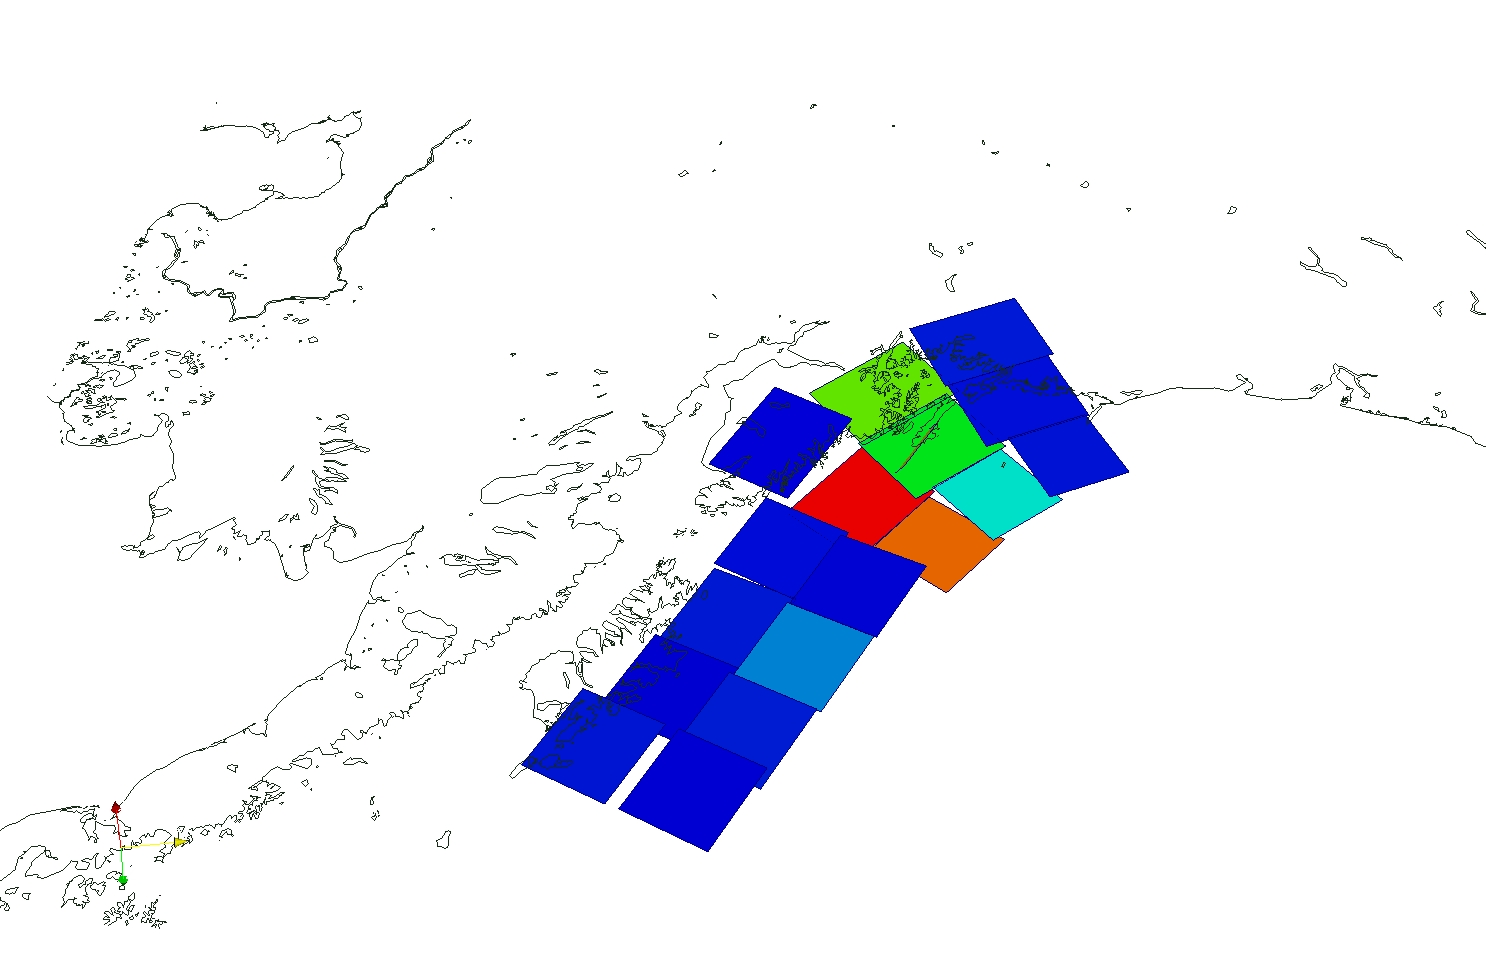
\includegraphics[width=\textwidth]{alaska.jpg}
\caption{\small Coseismic slip distribution of the 1964 M$_w$ 9.2 Alaska earthquake~\citep{johnson+96}. The utility 'flt2vtk.sh' transforms the slip distribution in the Paraview format for visualization in three dimensions.}
\label{fig:alaska}
\end{figure*}
%




\pagebreak
\section{Outputs}

All GMT output files related to a specific time step are prefixed by the index number, for instance \verb'000-east.grd' is the map view of the east component of deformation for index $0$. For each time step, for example index $14$, one can find\\
\\
\begin{tabular}{ll}
\verb'014-north.grd' & map view of the north component of cumulative displacement\\
\verb'014-east.grd' & map view of the east component of cumulative displacement\\
\verb'014-up.grd' & map view of the vertical component of cumulative displacement\\
\verb'014-relax-north.grd' & map view of the north component of postseismic displacement\\
\verb'014-relax-east.grd' & map view of the east component of postseismic displacement\\
\verb'014-relax-up.grd' & map view of the vertical component of postseismic displacement\\
\verb'014-s11.grd' & map view of the $\sigma_{11}$ component of cumulative stress\\
\verb'014-s12.grd' & map view of the $\sigma_{12}$ component of cumulative stress\\
\verb'014-s13.grd' & map view of the $\sigma_{13}$ component of cumulative stress\\
\verb'014-s22.grd' & map view of the $\sigma_{22}$ component of cumulative stress\\
\verb'014-s23.grd' & map view of the $\sigma_{23}$ component of cumulative stress\\
\verb'014-s33.grd' & map view of the $\sigma_{33}$ component of cumulative stress\\
\end{tabular}\\
\\
The export to files in the GMT binary format \verb'.grd' can be cancelled for the interest of space with the \verb'--no-grd-output' option.

All VTK output files for visualization in Paraview are suffixed with the output index numbers, for example \verb'sigma-0014.vtk'. For each time step, for instance index $14$, one can find\\
\\
\begin{tabular}{ll}
\verb'disp-0014.vtk' & subsampled volume of displacement vector\\
\verb'vel-0014.vtk' & subsampled volume of velocity vector\\
\verb'sigma-0014.vtk' & subsampled volume of stress tensor\\
\verb'power-0014.vtk' & subsampled volume of power tensor\\
\verb'disp-relax-0014.vtk' & subsampled volume of the relaxation part of the displacement vector (no coseismic)\\
\end{tabular}\\
\\
The output \verb'disp-relax-????.vtk' are only available with the \verb`--with-vtk-relax-output` option. The export to files in the VTK binary format \verb'.vtk' can be cancelled for the interest of space with the \verb'--no-vtk-output' option.

Some other files only contain geometrical information, such as geometry of fault patches, grid dimension, position of observation points:\\
\\
\begin{tabular}{ll}
\verb'opts.dat' & list of observation points (coordinates and names)\\
\verb'rfaults-001.xy' & GMT file containing the slip distribution of event 1\\
\verb'rfaults-001.vtp' & Paraview file containing the slip distribution of event 1\\
\verb'rfaults-dsigma-0014.vtp' & Paraview file containing the postseismic Coulomb stress for time step 14\\
\verb'rfaults-sigma-0014.vtp' & Paraview file containing the Coulomb stress for time step 14\\
\verb'aplane-0001.vtp' & Paraview file for the afterslip plane number 1\\
\verb'linearlayer-001.vtp' & Paraview file for depth of the first linear viscosity change\\
\verb'cgrid.vtp' & Paraview file for extent of the computational domain\\
\verb'weakzones-linear.vtp'  & Paraview file for all linear ductile zones\\
\verb'weakzones-nonlinear.vtp' & Paraview file for all nonlinear ductile zones\\
\verb'time.txt' &  time associated with time step\\
\end{tabular}\\

The time series of stress and displacement for observation points are in files \verb'NAME.txt'.







\pagebreak
\section{Benchmarks}

The numerical solution produced by Relax has been compared to many other analytical and numerical solutions. Here, we show two examples for static and time-dependent deformation. In general, it is a good practice to setup simulations using the most resource possible (the largest meshes, the smallest sampling).

\subsection{Coseismic deformation}
%
\begin{figure*}[h]
\centering
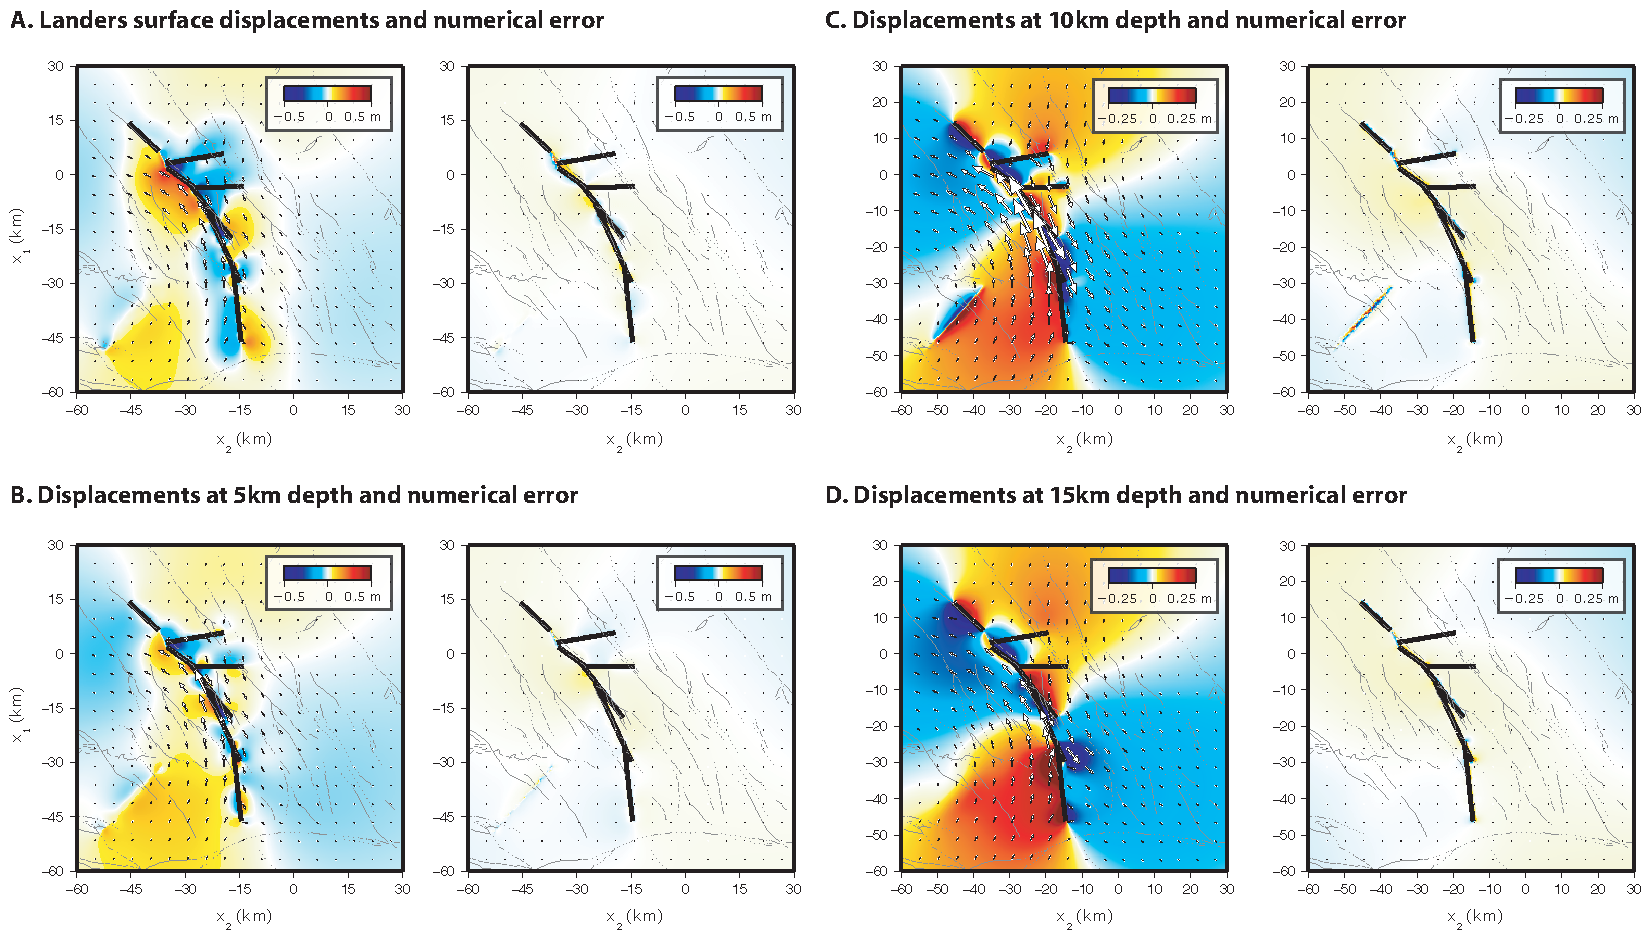
\includegraphics[width=\textwidth]{bm_landers.pdf}
\caption{\small Simulation of the 1992 Mw 7.3 Landers, CA earthquake. Comparison between the Relax numerical solution and the solution obtained with the \cite{okada92} Green's function at the surface (A), and at 5\,km (B), 10\,km (C) and 15\,km depth (D). For each depth the Relax solution is shown (left) and the residuals with \cite{okada92}. The arrows indicate horizontal displacement and the color represent vertical displacement (positive up). }
\label{fig:bm_landers}
\end{figure*}
%
Let's consider the coseismic deformation caused by the 1992 Mw 7.3 Landers, CA earthquake. Let's use the slip distribution of~\citep{fi04c}, which consists in 426 slip patches
\begin{alltt}
...
# number of shear dislocations
{\color{orange}426}
# index slip x1 x2 x3 length width strike dip rake
{\color{orange}1 1.3475 14.246 -45.439 10.056 5.6 4.94 132.7 91.0 -114.7
2 1.8921 10.446 -41.319 10.056 5.6 4.94 132.7 91.0 -151.8
3 0.46688 14.201 -45.481 6.5269 3.74 3.53 132.7 91.0 -150.6
4 0.38986 11.668 -42.734 6.5269 3.74 3.53 132.7 91.0 -175.6
5 1.3331 9.1346 -39.987 6.5269 3.74 3.53 132.7 91.0 172.8}
...
\end{alltt}
The corresponding input file can be found in the \verb'examples' directory in the file \verb'landers.sh'. Figure~\ref{fig:bm_landers} shows the comparison between the calculation with Relax on a $512^3$ grid with a sampling of $\Delta x=0.6\,$km and the analytic solution obtained with the~\cite{okada92} Green's function at various depths. The residuals maps reveals some numerical errors in the near field of the rupture caused by the equivalent body-force representation. Some long wavelength error appear at depth (\ref{fig:bm_landers}c,d) caused by the periodicity of the numerical solution due to the Fourier transform method. Overall the residuals are very small, demonstrating the possibility to model accurately geometrically complex earthquake ruptures.


\subsection{Non-linear viscoelastic relaxation}
Let's look at the postseismic relaxation due to the stress perturbation caused by dip-slip faulting, assuming uniform and isotropic elastic properties for a Poisson's solid (the Lam{\'e} parameters are such that $\lambda=G$ and Poisson's ratio is $\nu=1/4$). The fault slips 1\,m uniformly from the surface to a depth of 10\,km and is 40\,km long. We consider the case of a nonlinear viscoelastic upper mantle governed by the power-law rheology with $n=2$. We perform the computation with Relax in a $512^3$ grid with a uniform sampling of $\Delta x=0.8\,$km. A snapshot of the surface displacement early in the postseismic transient is shown in Figure~\ref{fig:bm_dslip_nonlin_2}a. The vertical postseismic displacement has the same polarity as the coseismic displacement. Horizontal postseismic displacements, however, are directed opposite to the coseismic ones. We performed the same simulation using the finite-element software Abaqus and the residuals are shown in the right panel of Figure~\ref{fig:bm_dslip_nonlin_2}a. The time series of surface postseismic displacements at points numbered from 1 to 8 in the maps are shown in Figure~\ref{fig:bm_dslip_nonlin_2}b. There is an excellent agreement between the semi-analytic and the finite-element results. The time series are characterized by two striking features. First, initial postseismic velocities are much higher than at later times, as most visible for points 1 and 2. Second, a change in polarity occurs at far-field locations. The change of postseismic displacement orientation is most flagrant for point 6 in the East-West direction. A mild change of polarity can be misleadingly interpreted as a delayed postseismic transient, as for the vertical displacement of point 8, for example.
%
\begin{figure*}
\begin{center}
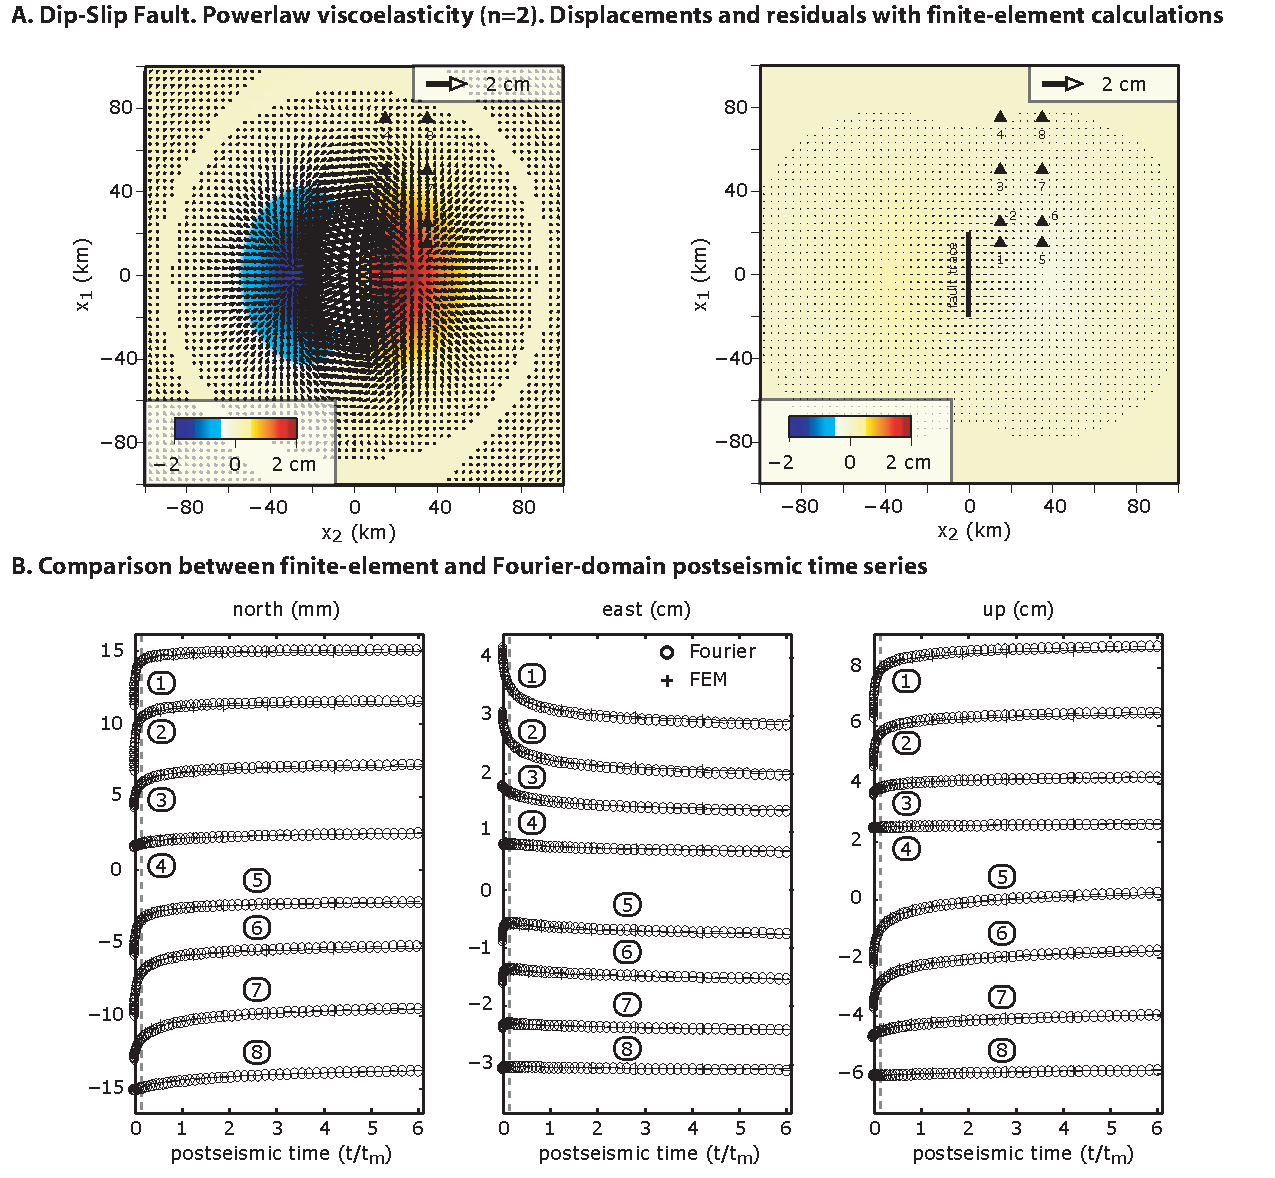
\includegraphics[width=\textwidth]{bm_dslip_nonlin_2.pdf}
\end{center}
\small
\caption{Benchmark for time series of surface displacement due to a stress perturbation caused by a dip-slip fault in an elastic plate overriding a nonlinear viscoelastic half space. A vertical dip-slip fault 40\,km long extending from the surface to a depth of 10\,km slips 1\,m. The brittle-ductile transition occurs at a depth of 30\,km. The postseismic flow is governed by a power-law rheology with stress exponent $n=2.0$. Elastic properties are uniform with $\nu=1/4$. A) A map view of postseismic surface displacements after ten months. A similar computation is performed using finite elements with Abaqus and the residuals are shown in the right panel. B) Time series of surface displacements for the points numbered from 1 to 8 in the corresponding map. The smaller time steps near the onset of the postseismic transient are due to the adaptative time-step procedure. Results from our approach are shown every 5 computation steps for clarity. The residuals between results from our numerical approach and the finite element calculation are less than 5\% and show reasonable agreement both in map view and in time.}
\label{fig:bm_dslip_nonlin_2}
\end{figure*}
%

\pagebreak
\section{Using Paraview with Relax}

This section offers a short introduction to using \verb`Paraview` to visualize three-dimensional objects and simulations. \verb`Paraview` also offers a convenient way to check the geometry of the models, including the input slip models and the relative position of other boundaries (viscous layers, ductile zone anomalies, receiver stress faults for Coulomb stress calculation). 

The first example uses the output created by the Coulomb stress calculation in the \verb`examples/mojave` directory. To run the example, type
\begin{verbatim}
cd examples/mojave
./coulomb.sh
\end{verbatim}
in a terminal. You can interrupt the program after this line appears
\begin{verbatim}
coseismic event 001
 I  |   Dt   | tm(ve) | tm(pl) | tm(as) |     t/tmax     | power  |  C:E^i |
000* 0.00E+00 0.00E+00 0.00E+00 0.00E+00 0.00E+00/2.00E+1 0.00E+00 3.60E+03
\end{verbatim}
as we only need the coseismic model. Figures~\ref{fig:cgrid-1} to \ref{fig:coulomb} show the procedure to import and visualize the model. First, load the computational extent of the model (Figs.~\ref{fig:cgrid-1} and \ref{fig:cgrid-2}). Then, load the source patches of the deformation (Fig.~\ref{fig:rfaults}). Use the \verb`Rescale to Data Range` and/or \verb`Edit Color Map...` controls in the \verb`Display` tab, if necessary. When running your first models, these first steps are a good way to verify the accuracy of the input geometry. Lastly, load the receiver faults and adjust the color scale (Fig.~\ref{fig:coulomb}). The stress calculation includes several projections of the stress tensor at the receiver fault location, including normal, shear and Coulomb stress, shear stress in the strike and dip direction, and the full stress tensor. Additional post-processing calculations can be done with the \verb`Calculator` filter.

The second example uses a model of the viscoelastic relaxation that follows the 1992 Mw 7.3 Landers earthquake. To run the simulation with the \verb`Paraview` output, type
\begin{verbatim}
./landers.sh --with-vtk-output --with-vtk-relax-output
\end{verbatim}
The first option, \verb`--with-vtk-output`, enforces the output in \verb`vtk` format, which is cancelled in \verb`landers.sh`; the second option, \verb`--with-vtk-relax-output` exports the relaxation contribution for three-dimensional visualization. The relaxation contribution is the total deformation, both elastic and viscoelastic, minus the coseismic deformation. This example also produces the output of the first one, so it is possible to reproduce the same steps. Additionally, you can load the three-dimensional coseismic displacement field (\verb`disp-..vtk`), and create the vector field using the \verb`Glyph` filter (Figs.~\ref{fig:disp-1} and \ref{fig:disp-2}). To look at the relaxation component, load \verb`disp-relax-..vtk`. You can then directly create a vector field, or you can decimate the data set to make the plot less dense (Fig.~\ref{fig:extract}). To plot the postseismic vector field, it is more convenient to move to another time step (postseismic component is zero by definition at time step zero). You can then apply the \verb`Glyph` filter on the data subset (Fig.~\ref{fig:disp-relax}). Finally, you can load the California faults trace or the UCERF three-dimensional fault model using the ancillary files located in \verb`examples/mojave/paraview`.



%
\begin{figure*}
\begin{center}
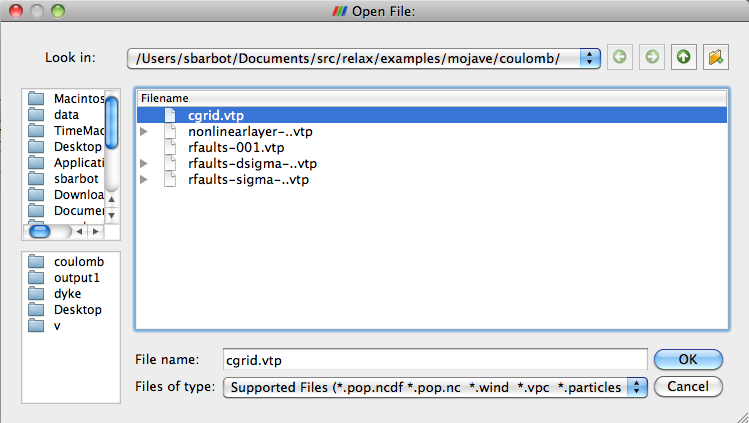
\includegraphics[width=\textwidth]{paraview-cgrid-1.png}
\end{center}
\small
\caption{Open the file containing the spatial extent of the computational domain.}
\label{fig:cgrid-1}
\end{figure*}
%

%
\begin{figure*}
\begin{center}
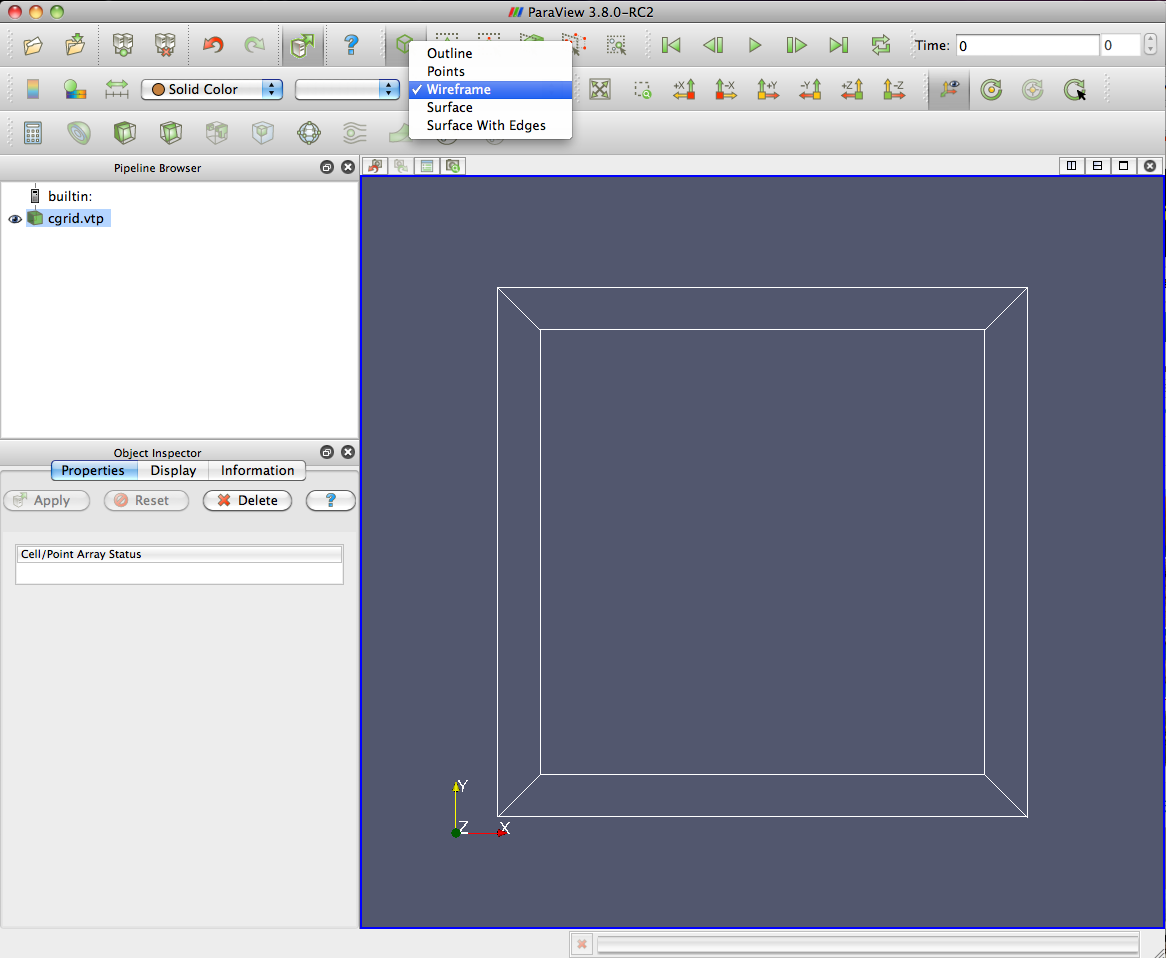
\includegraphics[width=\textwidth]{paraview-cgrid-2.png}
\end{center}
\small
\caption{Change the representation to wireframe to display online the boundary of the rectangular volume.}
\label{fig:cgrid-2}
\end{figure*}
%

%
\begin{figure*}
\begin{center}
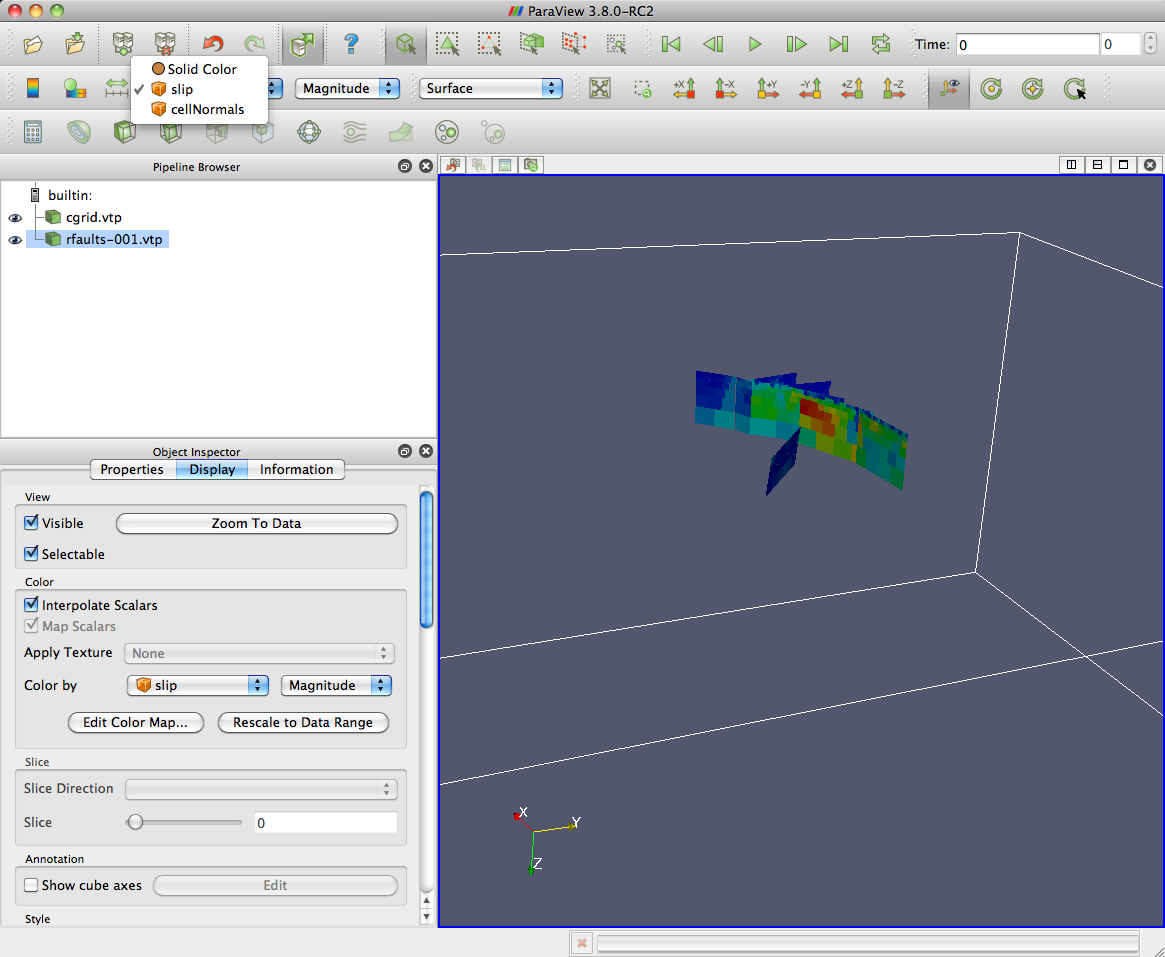
\includegraphics[width=\textwidth]{paraview-rfaults.png}
\end{center}
\small
\caption{Load the Landers slip model and color by the amplitude of slip. Rescale to data range in the ``display'' menu, if necessary.}
\label{fig:rfaults}
\end{figure*}
%

%
\begin{figure*}
\begin{center}
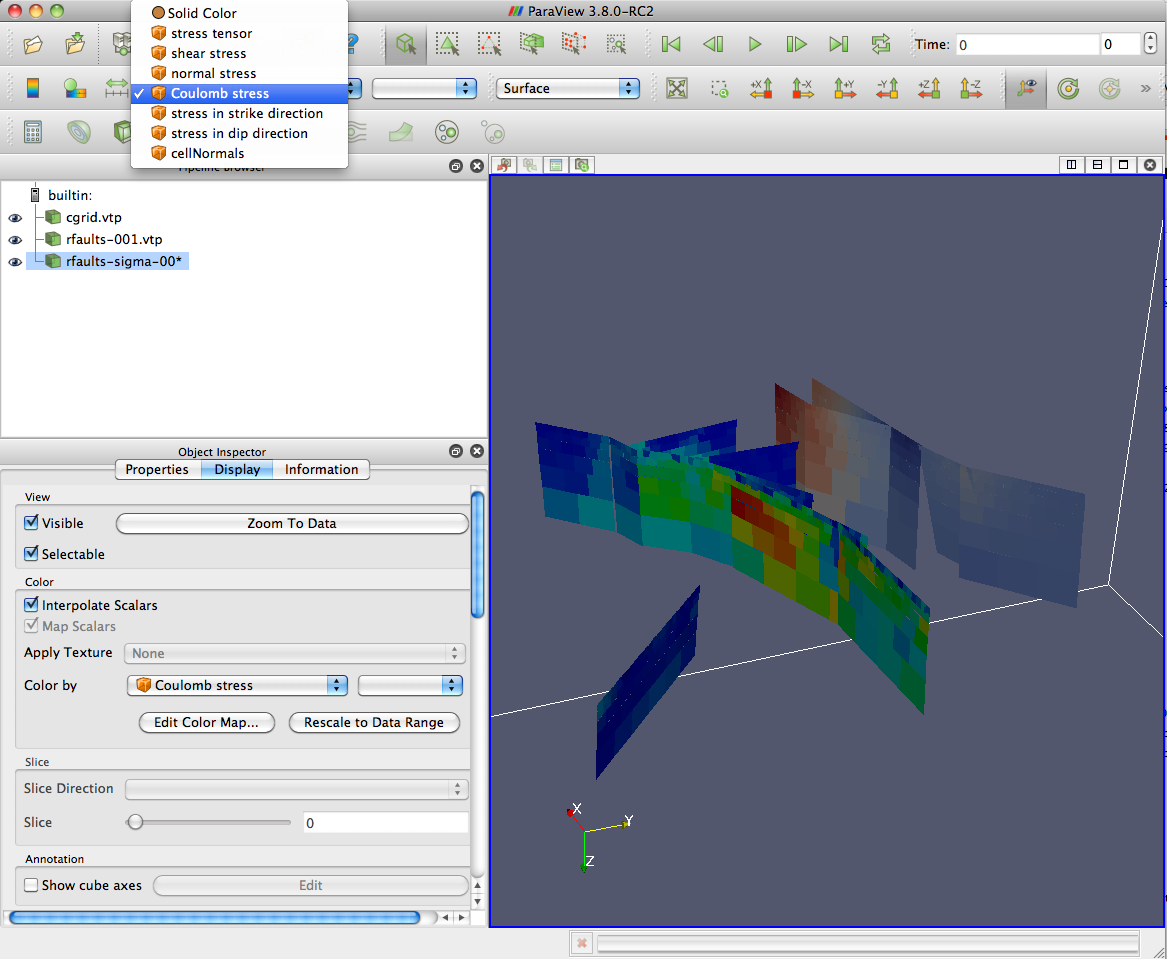
\includegraphics[width=\textwidth]{paraview-coulomb.png}
\end{center}
\small
\caption{Load the receiver faults, in the case the Hector Mine ruptured faults, and color by one in: shear, normal, Coulomb, strike-direction shear, dip-direction shear stresses. Rescale to data range in the ``Display'' window, if necessary.}
\label{fig:coulomb}
\end{figure*}
%


%
\begin{figure*}
\begin{center}
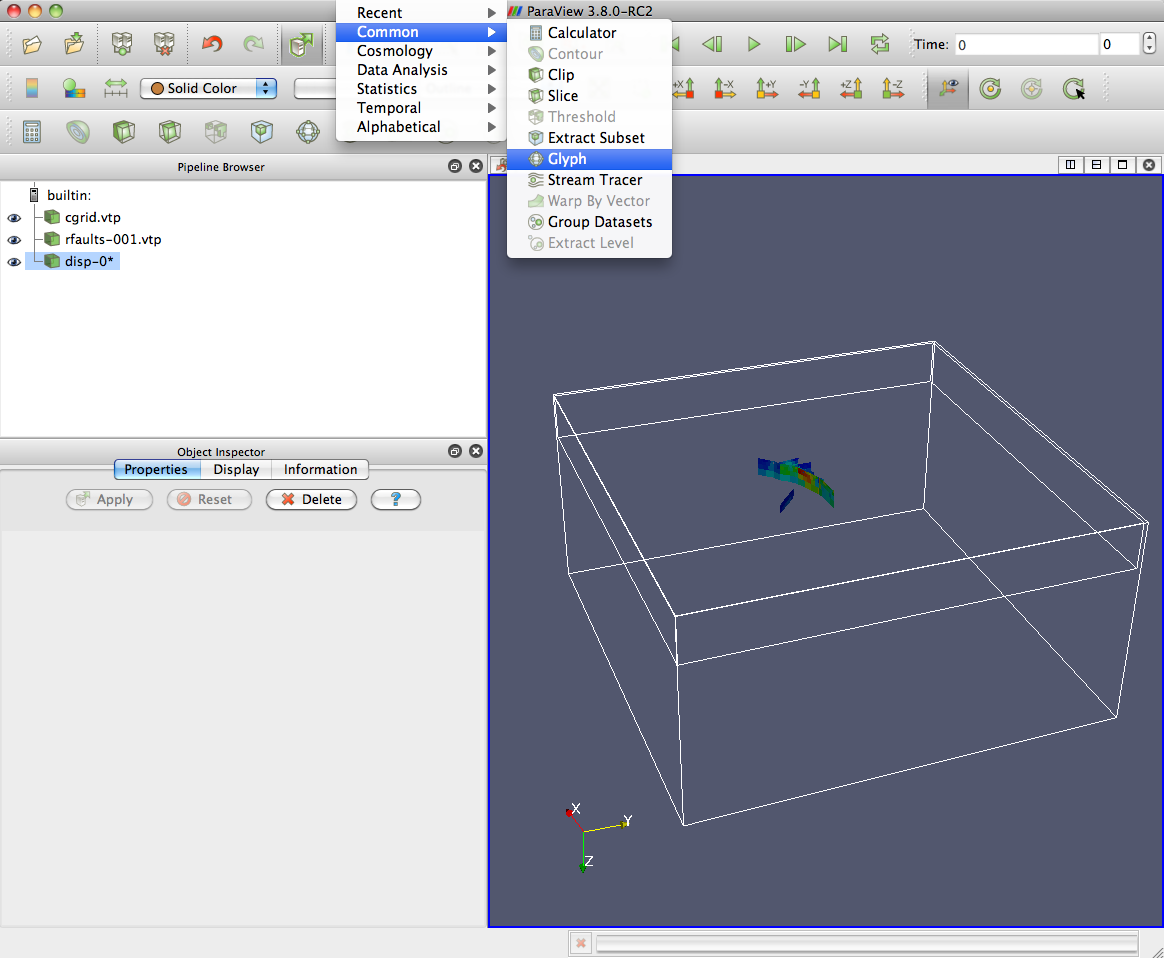
\includegraphics[width=\textwidth]{paraview-disp-1.png}
\end{center}
\small
\caption{Load the displacement field (disp-0* appears on the ``Pipeline Browser'') and apply the ``Glyph'' filter.}
\label{fig:disp-1}
\end{figure*}
%

%
\begin{figure*}
\begin{center}
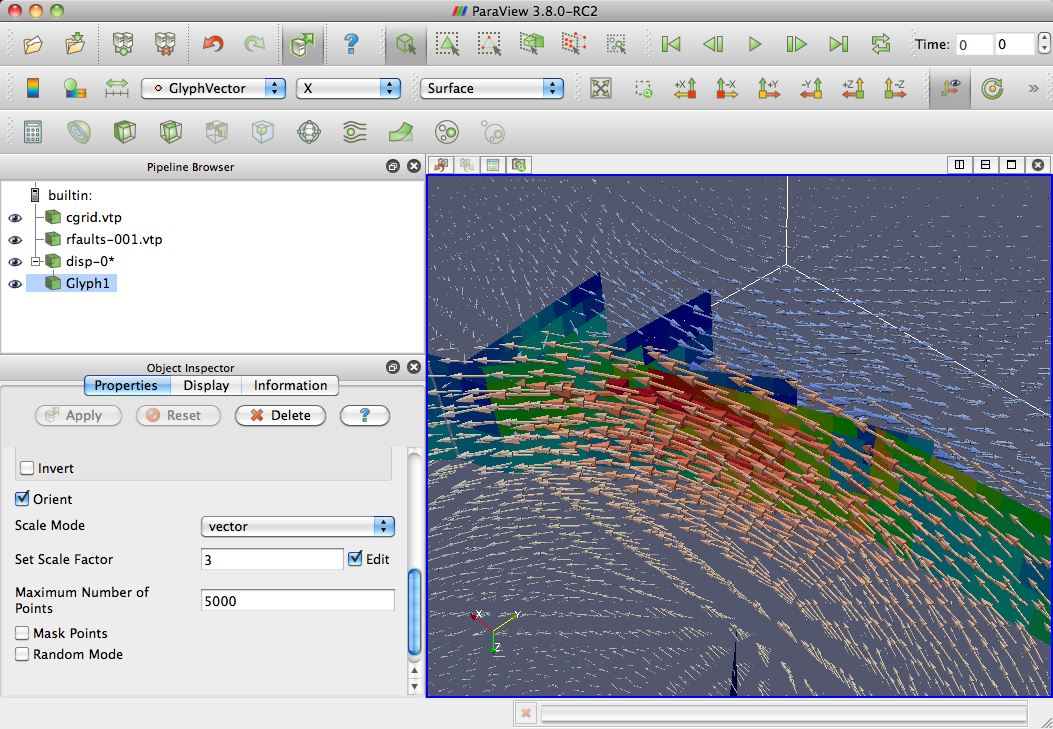
\includegraphics[width=\textwidth]{paraview-disp-2.png}
\end{center}
\small
\caption{Adjust the scale factor, points masking and random mode and set the color to ``GlyphVector''.}
\label{fig:disp-2}
\end{figure*}
%

%
\begin{figure*}
\begin{center}
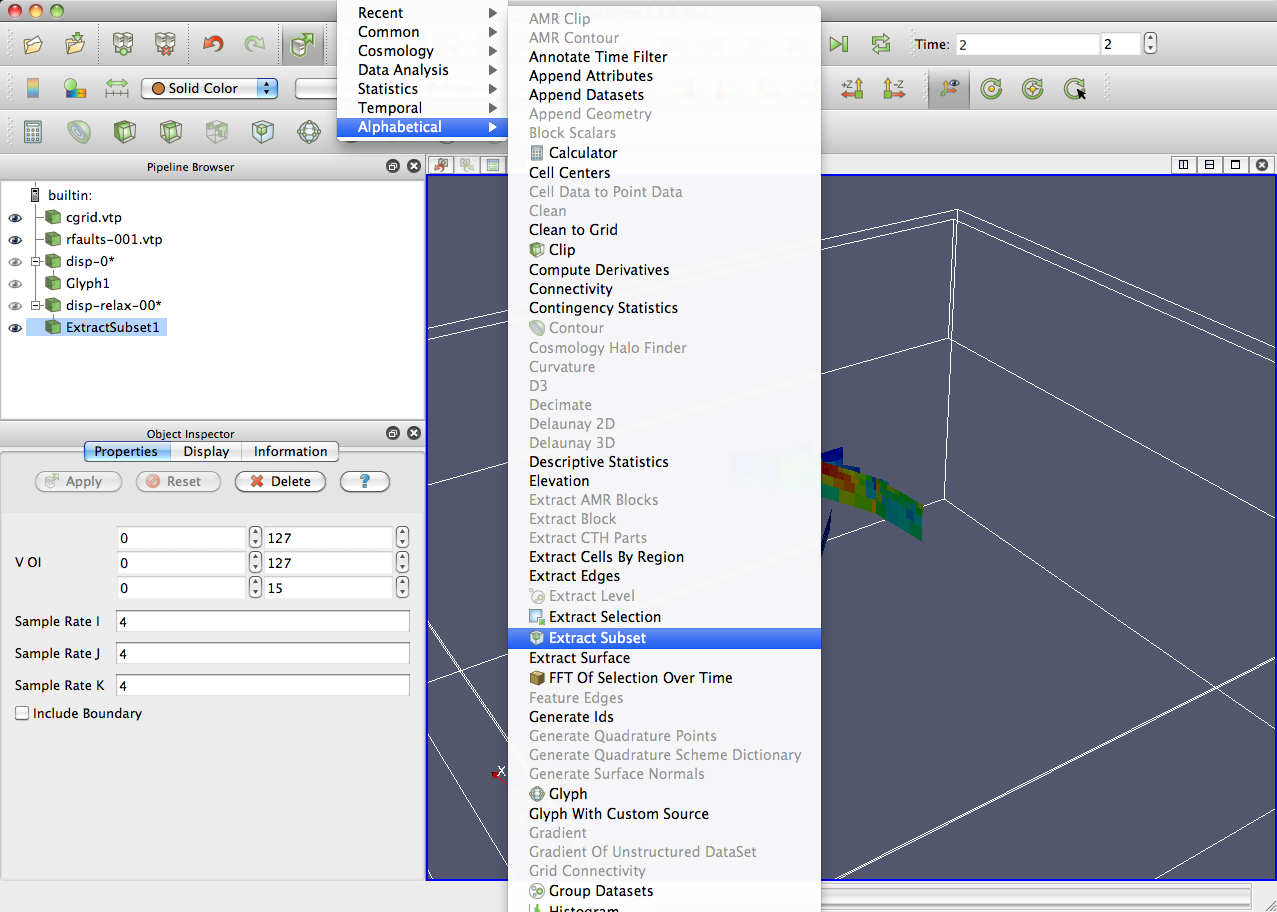
\includegraphics[width=\textwidth]{paraview-extract.png}
\end{center}
\small
\caption{Load the relaxation component of the deformation (``disp-relax-0*'' appears on the ``Pipeline Browser''), then decimate the data set to prepare for a larger displacement field vector. To take one every four points, adjust the ``Sample Rate I'' accordingly.}
\label{fig:extract}
\end{figure*}
%

%
\begin{figure*}
\begin{center}
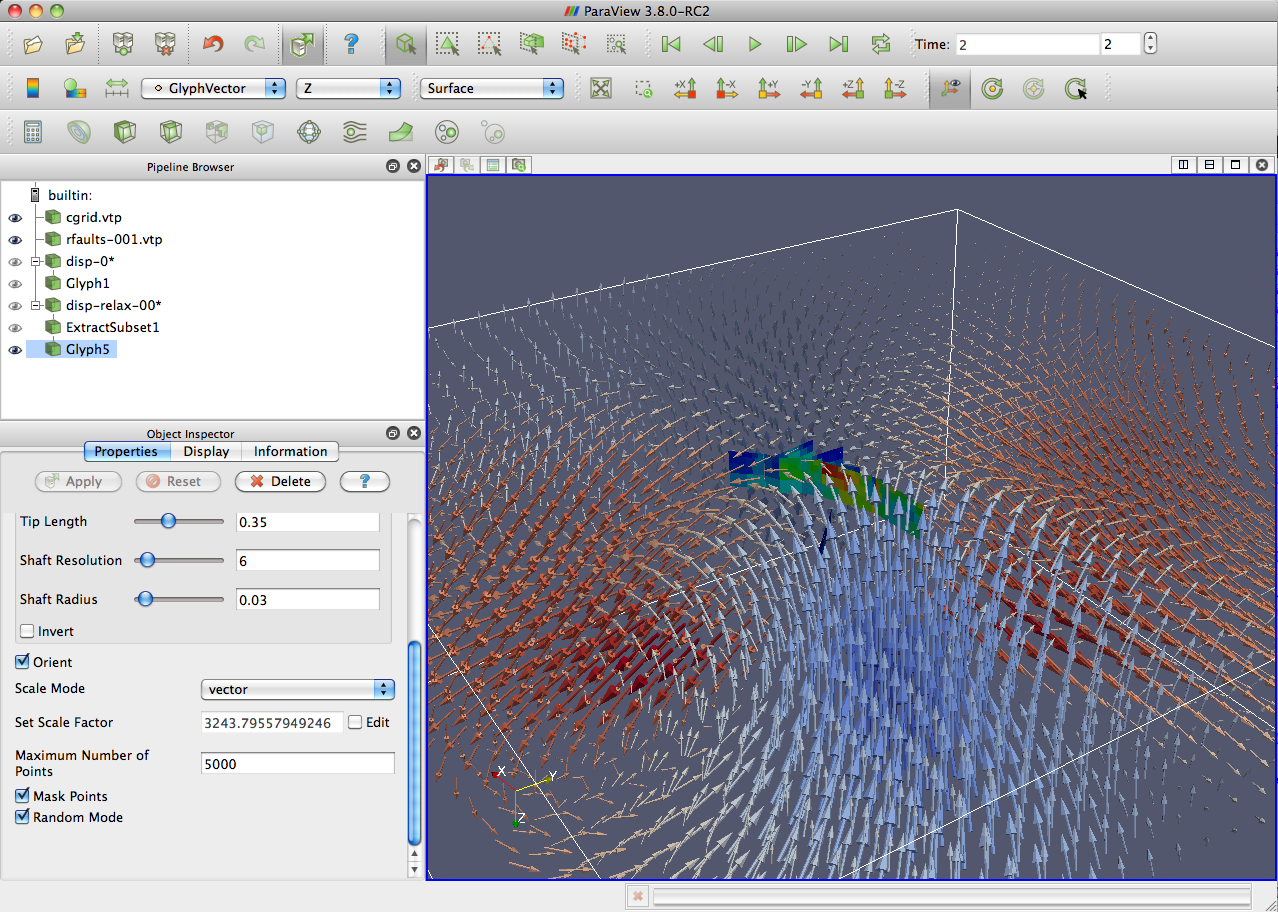
\includegraphics[width=\textwidth]{paraview-disp-relax.png}
\end{center}
\small
\caption{Apply the ``Glyph'' filter on the ``ExtractSubset1'' new data set, then change the color scale to ``GlyphVector'' and cancel the visibility of the ``ExtractSubset1'', the ``disp-relax-00*'' datasets (check out the eye controls).}
\label{fig:disp-relax}
\end{figure*}
%

\pagebreak
%\bibliography{../../../latex/reference}
\bibliographystyle{agu}

\begin{thebibliography}{20}
\providecommand{\natexlab}[1]{#1}
\expandafter\ifx\csname urlstyle\endcsname\relax
  \providecommand{\doi}[1]{doi:\discretionary{}{}{}#1}\else
  \providecommand{\doi}{doi:\discretionary{}{}{}\begingroup
  \urlstyle{rm}\Url}\fi

\bibitem[{\textit{Aki and Richards}(1980)}]{aki&richards80a}
Aki, K., and P.~G. Richards, \textit{Quantitative Seismology}, vol.~I, W. H.
  Freeman and company, New York, 1980.

\bibitem[{\textit{Barbot and Fialko}(2010{\natexlab{a}})}]{barbot&fialko10a}
Barbot, S., and Y.~Fialko, Fourier-domain {G}reen function for an elastic
  semi-infinite solid under gravity, with applications to earthquake and
  volcano deformation, \textit{Geophys. J. Int.}, \textit{182}(2), 568�582,
  \doi{10.1111/j.1365-246X.2010.04655.x}, 2010{\natexlab{a}}.

\bibitem[{\textit{Barbot and Fialko}(2010{\natexlab{b}})}]{barbot&fialko10b}
Barbot, S., and Y.~Fialko, A unified continuum representation of postseismic
  relaxation mechanisms: semi-analytic models of afterslip, poroelastic rebound
  and viscoelastic flow, \textit{Geophys. J. Int.}, \textit{182}(3),
  1124--1140, \doi{10.1111/j.1365-246X.2010.04678.x}, 2010{\natexlab{b}}.

\bibitem[{\textit{Barbot et~al.}(2009{\natexlab{a}})\textit{Barbot, Fialko, and
  Bock}}]{barbot+09a}
Barbot, S., Y.~Fialko, and Y.~Bock, {Postseismic Deformation due to the Mw\,6.0
  2004 Parkfield Earthquake: Stress-Driven Creep on a Fault with Spatially
  Variable Rate-and-State Friction Parameters}, \textit{J. Geophys. Res.},
  \textit{114}(B07405), \doi{10.1029/2008JB005748}, 2009{\natexlab{a}}.

\bibitem[{\textit{Barbot et~al.}(2009{\natexlab{b}})\textit{Barbot, Fialko, and
  Sandwell}}]{barbot+09b}
Barbot, S., Y.~Fialko, and D.~Sandwell, {Three-Dimensional Models of
  Elasto-Static Deformation in Heterogeneous Media, with Applications to the
  Eastern California Shear Zone}, \textit{Geophys. J. Int.}, \textit{179}(1),
  500--520, 2009{\natexlab{b}}.

\bibitem[{\textit{Bruhat et~al.}(2011)\textit{Bruhat, Barbot, and
  Avouac}}]{bruhat+11}
Bruhat, L., S.~Barbot, and J.~P. Avouac, {Evidence for postseismic deformation
  of the lower crust following the 2004 Mw6.0 Parkfield earthquake}, \textit{J.
  Geophys. Res.}, \textit{116}, 10, 2011.

\bibitem[{\textit{Elliott et~al.}(2010)\textit{Elliott, Walters, England,
  Jackson, Li, and Parsons}}]{elliott+10}
Elliott, J.~R., R.~J. Walters, P.~C. England, J.~A. Jackson, Z.~Li, and
  B.~Parsons, {Extension on the Tibetan plateau: recent normal faulting
  measured by InSAR and body wave seismology}, \textit{Geophys. J. Int.},
  \textit{183}(2), 503�535, 2010.

\bibitem[{\textit{Elliott et~al.}(2012)\textit{Elliott, Nissen, England,
  Jackson, Lamb, Li, Oehlers, and Parsons}}]{elliott+12}
Elliott, J.~R., E.~K. Nissen, P.~C. England, J.~A. Jackson, S.~Lamb, Z.~Li,
  M.~Oehlers, and B.~Parsons, {Slip in the 2010-2011 Canterbury earthquakes,
  New Zealand}, \textit{J. Geophys. Res.}, \textit{117}(B03401), 36, 2012.

\bibitem[{\textit{Fialko}(2004)}]{fi04c}
Fialko, Y., {Evidence of fluid-filled upper crust from observations of
  post-seismic deformation due to the 1992 M$_w$7.3 Landers earthquake},
  \textit{J. Geophys. Res.}, \textit{109}, B08,401, 10.1029/2004JB002,985,
  2004.

\bibitem[{\textit{Johnson et~al.}(1996)\textit{Johnson, Satake, Holdahl, and
  Sauber}}]{johnson+96}
Johnson, J.~M., K.~Satake, S.~R. Holdahl, and J.~Sauber, {The 1964 Prince
  William Sound earthquake: Joint inversion of tsunami and geodetic data},
  \textit{J. Geophys. Res.}, \textit{101}(B1), 523--532, 1996.

\bibitem[{\textit{Johnson et~al.}(2001)\textit{Johnson, Hsu, Segall, and
  Yu}}]{johnson+01}
Johnson, K.~M., Y.~J. Hsu, P.~Segall, and S.~B. Yu, Fault geometry and slip
  distribution of the 1999 chi-chi, taiwan earthquake imaged from inversion of
  gps data, \textit{Geophys. Res. Lett}, \textit{28}(11), 2285--2288, 2001.

\bibitem[{\textit{Lasserre et~al.}()\textit{Lasserre, Peltzer, Cramp\'{e},
  Klinger, der Woerd, and Tapponnier}}]{lasserre+05}
Lasserre, C., G.~Peltzer, F.~Cramp\'{e}, Y.~Klinger, J.~V. der Woerd, and
  P.~Tapponnier.

\bibitem[{\textit{Li et~al.}(2011)\textit{Li, Elliott, Feng, Jackson, Parsons,
  and Walters}}]{li+11}
Li, Z., J.~R. Elliott, W.~Feng, J.~A. Jackson, B.~E. Parsons, and R.~J.
  Walters, {The 2010 MW 6.8 Yushu (Qinghai, China) earthquake: Constraints
  provided by InSAR and body wave seismology}, \textit{J. Geophys. Res.},
  \textit{116}(B10302), 16, 2011.

\bibitem[{\textit{Mogi}(1958)}]{mogi58}
Mogi, K., Relations between the eruptions of various volcanoes and the
  deformations of the ground surfaces around them, \textit{Bull. Earthquake
  Res. Inst. Univ. Tokyo}, \textit{36}, 99--134, 1958.

\bibitem[{\textit{Okada}(1992)}]{okada92}
Okada, Y., Internal deformation due to shear and tensile faults in a
  half-space, \textit{Bull. Seism. Soc. Am.}, \textit{82}, 1018--1040, 1992.

\bibitem[{\textit{Rousset et~al.}(2012)\textit{Rousset, Barbot, Avouac, and
 Hsu}}]{rousset+12}
Rousset, B., S.~Barbot, J.-P.~Avouac and Y.-J.~Hsu, {Postseismic deformation following the 1999 Chi-Chi earthquake, Taiwan: Implication for the lower-crust rheology}, \textit{J. Geophys. Res.}, \textit{117}, 2012.

\bibitem[{\textit{Ryder et~al.}(2011)\textit{Ryder, B\"{u}rgmann, and
  Pollitz}}]{ryder+11}
Ryder, I., R.~B\"{u}rgmann, and F.~Pollitz, {Lower crustal relaxation beneath
  the Tibetan Pleateau and Qaidam Basin following the 2001 Kokoxili
  earthquake}, \textit{Geophys. J. Int.}, \textit{187}, 613--630, 2011.

\bibitem[{\textit{Simons et~al.}(2002)\textit{Simons, Fialko, and
  Rivera}}]{si+02a}
Simons, M., Y.~Fialko, and L.~Rivera, {Coseismic deformation from the 1999
  $M_w7.1$ Hector Mine, California, earthquake, as inferred from InSAR and GPS
  observations}, \textit{Bull. Seism. Soc. Am.}, \textit{92}, 1390--1402, 2002.

\bibitem[{\textit{Wang et~al.}(2003)\textit{Wang, Martin, and Roth}}]{wang+03a}
Wang, R., F.~Martin, and F.~Roth, {Computation of deformation induced by
  earthquakes in a multi-layered elastic crust - FORTRAN programs EDGRN/EDCMP},
  \textit{Comp. Geosci.}, \textit{29}, 195--207, 2003.

\bibitem[{\textit{Wang et~al.}(2006)\textit{Wang, Lorenzo-Martin, and
  Roth}}]{wang+06a}
Wang, R., F.~Lorenzo-Martin, and F.~Roth, {PSGRN/PSCMP}-a new code for
  calculating co- and post-seismic deformation, geoid and gravity changes based
  on the viscoelastic-gravitational dislocation theory, \textit{Computers and
  Geosciences}, \textit{32}, 527--541, 2006.

\end{thebibliography}



\clearpage


\end{document}
